%### New page ############################################################

%%%%\begin{frame}[fragile]
%%%%
%%%%\frametitle{``Push through'' uncertainty}
%%%%
%%%%\begin{center}
%%%%\rotatebox{0}{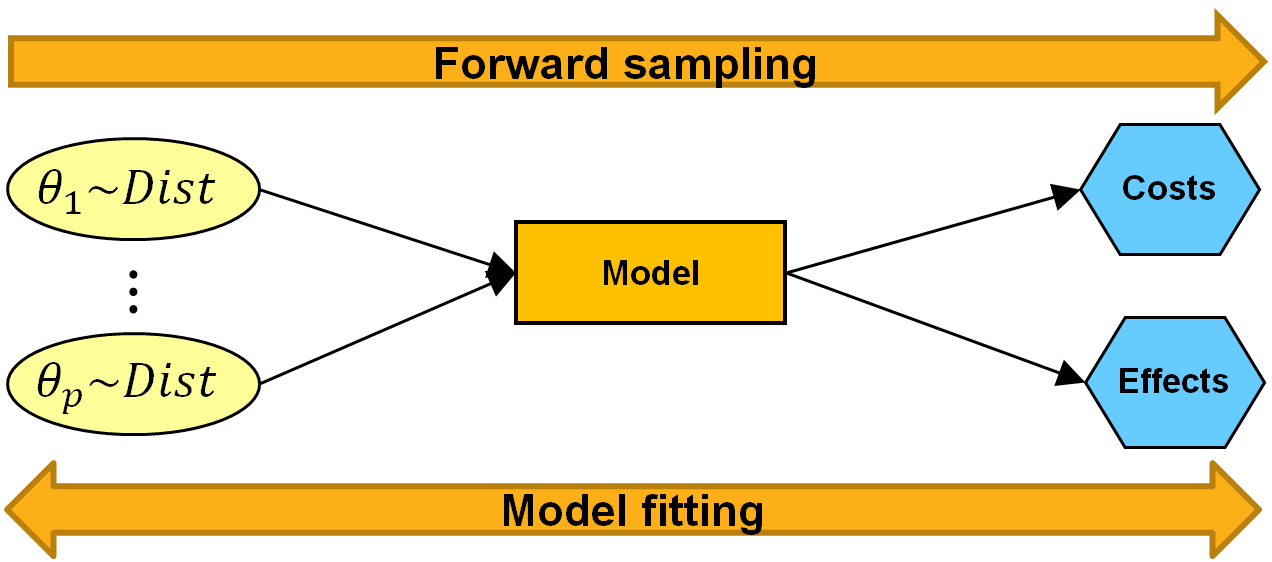
\includegraphics[height=4.5cm]{6.probabilistic-sensitivity-analysis/figs/forward_backward.png}}
%%%%\end{center}
%%%%
%%%%\end{frame}

\begin{frame}
\frametitle{``Push through'' uncertainty}
\begin{center}
\begin{tikzpicture}
\tikzset{>={Triangle[width=10mm,length=10mm]}}
\node [ellipse,minimum height=8mm,inner sep=0pt,outer sep=0pt,fill=yellow!40!white,draw] at (-3,2) (rand1) {$\theta_1 \sim \mbox{Distr}$};
\node [ellipse,minimum height=8mm,inner sep=0pt,outer sep=0pt,fill=yellow!40!white,draw] at (-3,-0) (rand2) {$\theta_P \sim \mbox{Distr}$};
\node [rectangle,minimum height=8mm,minimum width=18mm,inner sep=0pt,outer sep=0pt,fill=orange!70!white,draw,thick] at (1,1) (model) {Model};
\node[regular polygon,regular polygon sides=6,minimum width=16mm,inner sep=0pt,outer sep=0pt,fill=blue!30!white,draw] at (5,2) (util1) {Costs};
\node[regular polygon,regular polygon sides=6,minimum width=16mm,inner sep=0pt,outer sep=0pt,fill=blue!30!white,draw] at (5,-0) (util2) {Effects};
\node [inner sep=0pt,outer sep=0pt] at (-3,1) (dots) {$\vdots$};

\draw [->,>=latex,shorten >=0pt,auto,node distance=0cm,thin,color=black] (rand1.-5) to (model.170);
\draw [->,>=latex,shorten >=0pt,auto,node distance=0cm,thin,color=black] (rand2.5) to (model.190);
\draw [->,>=latex,shorten >=0pt,auto,node distance=0cm,thin,color=black] (model.-5) to (util2.180);
\draw [->,>=latex,shorten >=0pt,auto,node distance=0cm,thin,color=black] (model.5) to (util1.180);
\draw [->,>={Triangle[width=12mm,length=12mm]},orange!100!white,line width=18pt]  (-4,3.5) to node[black]{} (6.1,3.5) ;
\draw [->,orange!70!white, line width=15pt]  (-3.95,3.5) to node[black]{\textbf{Forward sampling}} (5.95,3.5) ;
\draw [->,>={Triangle[width=12mm,length=12mm]},orange!100!white,line width=18pt]  (6,-1.5) to node[black]{} (-4.1,-1.5) ;
\draw [->,orange!70!white,line width=15pt]  (5.95,-1.5) to node[black]{\textbf{Model fitting}} (-3.95,-1.5) ;
\end{tikzpicture}
\end{center}
\end{frame}

%### New page ############################################################

\begin{frame}

\frametitle{Summary}

\bi

\item One step parameter estimation and cost-effectiveness model
\bi
\item Set up a deterministic health economic model
\item Estimate parameters and ``push through'' the uncertainty in the parameters underpinning this model by Monte Carlo simulation
\ei

\item  This generates the distribution of the population mean effectiveness and population mean cost in each arm
\bi
\item $\mbox{E}[f(\theta)] \neq f \left( \mbox{E}[\theta] \right) $
\ei

\item We use these distributions to find
\bi
\item Incremental cost-effectiveness ratio
\item Incremental net benefit
\item Cost effectiveness acceptability curves
\ei
%%%
%%%\item We calculate the value of reducing the uncertainty in the parameters
%%%\bi
%%%\item Expected value of perfect information
%%%\item Expected value of perfect partial information
%%%\ei
\ei

\vfill
{\footnotesize  \emph{Bayesian Methods in Health Economics} (BMHE), chapter 3.4 -- 3.5}

\end{frame}


%### New page ############################################################

\begin{frame}

\frametitle{New chemotherapy drug}

\bi
\item Evaluate a new chemotherapy drug against the standard of care

\item Following treatment, a patient may experience haematological side effects

\item If this does happen, depending on the severity, the patient either needs ambulatory care, or is admitted to hospital

\item Costs to include: Drug costs, cost of ambulatory care, cost of hospital

\item Effect: Being free of side effects
\ei

\end{frame}

%### New page ############################################################

\begin{frame}

\frametitle{Components of Decision Quality\footnote{Ron Howard. \href{https://pdfs.semanticscholar.org/b86d/350c0207d1a3ebacc7910a1691e6c091ff46.pdf}{The Foundations of Decision Analysis Revisited}, in Advances in Decision Analysis 2007.}}

\bi
\item \textbf{What can we do?}
\bi
\item $t$ is the set of interventions
\item Decide to use standard-or-care or new treatment ($\myblue t = 1, 2$)
\ei\pause\vspace{5pt}

\item \textbf{What do we know?}
\bi
%%%\item Statistically these are the \alert{random variables}
\item $\myblue \bm{\theta}$: parameters describing  disease model, costs and effects
\item $\myblue e$ and $\myblue c$ are the observable outcomes
\item $\myblue \mu_t^e = \mbox{E}[e\mid\theta, t]$ and $\myblue \mu_t^c= \mbox{E}[c\mid\theta, t]$ are population mean cost and effect given intervention $t$.
\ei\pause\vspace{5pt}

\item \textbf{What do we want?}
\bi
\item The value of the outcomes, \alert{measured by utility}
\item We chose the \alert{net (monetary) benefit} $\myblue u(e,c;t) = ke-c$, where $k$ is the willingness-to-pay for one unit of effectiveness.
\item Chose intervention $t$ with the highest \textbf{expected net benefit}\\
%$\mbox{E}\left[ \mbox{E}[u(e,c;t)] \right] = \mbox{E}\left[k\mu_t^e-\mu_t^c \right]$\\
$\myblue \mbox{E}\left[\mbox{NB}_t(\bm\theta)\right] = \mbox{E}\left[k\mu_t^e-\mu_t^c \right] = \mbox{E}_{\bm\theta}\left[ \mbox{E}_{(e,c)}[u(e,c;t)] \right]$\\
\ei
\ei

\end{frame}

%%%%%%### New page ############################################################
%%%%%
%%%%%\begin{frame}
%%%%%
%%%%%\frametitle{Decision tree model}
%%%%%
%%%%%
%%%%%\begin{center}
%%%%%\rotatebox{0}{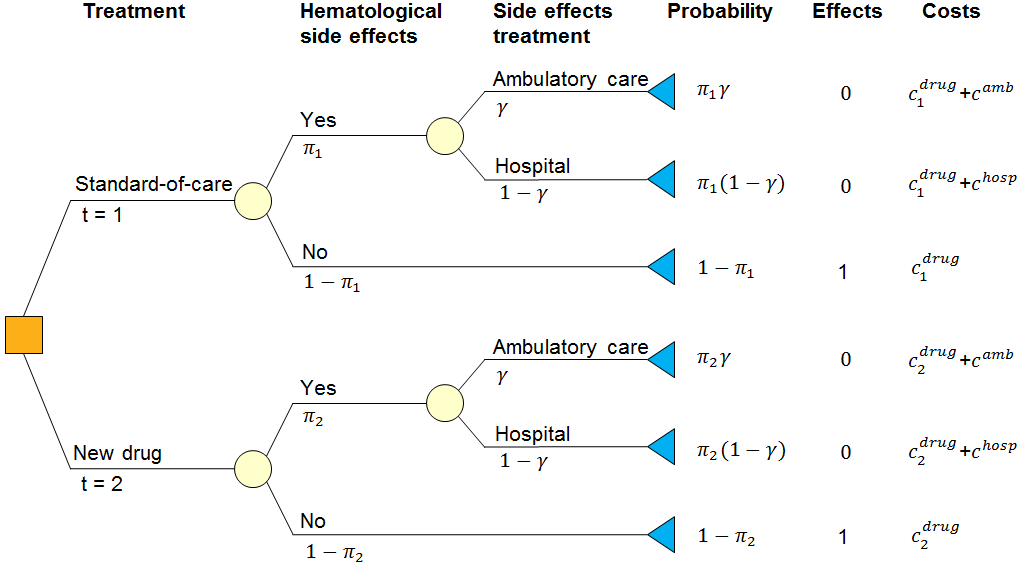
\includegraphics[height=6.5cm]{6.probabilistic-sensitivity-analysis/figs/chemo_decision_tree.png}}
%%%%%\end{center}
%%%%%
%%%%%
%%%%%\end{frame}


\begin{frame}

\frametitle{Decision tree model}

\centering
\begin{tikzpicture}
\draw(-6,1) node[align=center,draw=none,fill=none,minimum width=.5cm,minimum height=.5cm,font=\sffamily\fontsize{8}
{8}\selectfont](1){$\myblue N$\\ Standard \\treatment};

\draw(0,-1) node[align=center,draw=none,fill=none,minimum width=.5cm,minimum height=.5cm,font=\sffamily\fontsize{8}{9}\selectfont](2){$\myblue N-SE_t$\\ No side effects\\$\olive (1-\pi_t)$};

\draw(-3,3) node[align=center,draw=none,fill=none,minimum width=.5cm,minimum height=.5cm,font=\sffamily\fontsize{8}{9}\selectfont](3){$\myblue SE_t$\\ Blood-related \\side effects \\$\olive (\pi_t)$};

\draw(0,4) node[align=center,draw=none,fill=none,minimum width=.5cm,minimum height=.5cm,font=\sffamily\fontsize{8}{9}\selectfont](4){$\myblue A_t$\\ Ambulatory care \\$\olive (\gamma)$};

\draw(0,2) node[align=center,draw=none,fill=none,minimum width=.5cm,minimum height=.5cm,font=\sffamily\fontsize{8}{9}\selectfont](5){$\myblue SE_t-A_t$\\ Hospital admission \\$\olive (1-\gamma)$};

\draw(3,4.1) node[align=center,draw=none,fill=none,minimum width=.5cm,minimum height=.5cm,font=\sffamily\fontsize{8}{9}\selectfont](6){$\red e_t=0,c_t=c_t^{drug}+c^{amb}$};

\draw(3,2.1) node[align=center,draw=none,fill=none,minimum width=.5cm,minimum height=.5cm,font=\sffamily\fontsize{8}{9}\selectfont](7){$\red e_t=0,c_t=c_t^{drug}+c^{hosp}$};

\draw(3,-0.9) node[align=center,draw=none,fill=none,minimum width=.5cm,minimum height=.5cm,font=\sffamily\fontsize{8}{9}\selectfont](7){\red $e_t=1,c_t=c_t^{drug}$};

\draw(3,4.8) node[align=center,draw=none,fill=none,minimum width=.5cm,minimum height=.5cm,font=\sffamily\fontsize{8}{9}\selectfont](8){\underline{Economic outcomes}};

\node [circle,minimum size=2mm,inner sep=0pt,outer sep=0pt,fill=black] at (-5.25,1) (rand1){};
\node [circle,minimum size=2mm,inner sep=0pt,outer sep=0pt,fill=black] at (-2.04,3) (rand2){};

\draw [->,>=latex,shorten >=0pt,auto,node distance=3cm,ultra thin] (1.east) |- (2.west);
\draw [->,>=latex,shorten >=0pt,auto,node distance=3cm,ultra thin] (1.east) |- (3.west);
\draw [->,>=latex,shorten >=0pt,auto,node distance=3cm,ultra thin] (3.east) |- (4.west);
\draw [->,>=latex,shorten >=0pt,auto,node distance=3cm,ultra thin] (3.east) |- (5.west);
\end{tikzpicture}

\end{frame}


%### New page ############################################################

\begin{frame}

\frametitle{Disease model data}

We have data from a clinical study


\begin{center}
\small
\begin{tabular}{lrl}
\hline
Parameter  & Value & Description\\
\hline
$N^{pat}$ & 111 & Number of patients in observed data \\
$N^{se}$  & 27  & Number of patients with side effects,  \\ &&given standard-of-care \\
$N^{amb}$ & 17  & Number of patient with ambulatory care following \\ &&side effect, given standard-of-care \\
$\mu_{\rho}$ & 0.8  & Mean relative probability of side effects \\ &&in new treatment compared to standard-of-care \\
$\sigma_{\rho}$ & 0.2  & SE of relative probability of side effects \\ &&in new treatment compared to standard-of-care \\
\hline

\end{tabular}
\end{center}
\end{frame}

%### New page ############################################################

\begin{frame}[fragile]

\frametitle{Disease model analysis}

{\small
Probability of side effects

\begin{tabular}{ccll}
$N^{\rm{se}}$ & $\sim$ & $\mbox{Binomial}(\pi_1, N^{\rm{pat}})$         & sampling distribution \\
$\pi_1$           & $\sim$ & $\mbox{Beta}(1, 1)$                                & prior distribution \\
$\rho$            & $\sim$ & $\mbox{Normal}(\mu_{\rho}, \sigma_{\rho}^2)$ & Reduction in the occurence of side effects \\
$\pi_2$           & $=$    & $\rho \pi_1$                                      &  \\
\end{tabular}

Treatment of side effects

\begin{tabular}{ccll}
$N^{\rm{amb}}$ & $\sim$  & $\mbox{Binomial}(\gamma, N^{\rm{se}})$  & sampling distribution \\
$\mathtt{\gamma}$  &  $\sim$ & $\mbox{Beta}(1, 1)$                         & prior distribution \\
\end{tabular}

\begin{semiverbatim}
\olive
num.se \mytilde dbin(pi[1], num.pat)
pi[1] \mytilde dbeta(1, 1)

rho \mytilde dnorm(m.rho, tau.rho)
pi[2] <- rho * pi[1]

num.amb \mytilde dbin(gamma, num.se)
gamma \mytilde dbeta(1, 1)

\end{semiverbatim}
}

\end{frame}


%### New page ############################################################

\begin{frame}[fragile]

\frametitle{Cost Data}

{\footnotesize
\begin{center}
\begin{tabular}{lrll}
\hline
Parameter  & Distribution & Description & Mean cost\\
  \hline\\[-6pt]
  $c^{\rm{amb}}$ & logNormal(4.77, 0.17) & Ambulatory care & 120 \\
  $c^{\rm{hosp}}$ &  logNormal(8.60, 0.18) & Hospital & 5483 \\
  $c_1^{\rm{drug}}$ & 110  & Cost of standard-of-care \\
  $c_2^{\rm{drug}}$ & 520 & Cost of new drug \\
  \hline
\end{tabular}
\end{center}
}

\vfill 

{\small
\begin{semiverbatim}
\olive
c.amb \mytilde  dlnorm(m.amb, tau.amb)     # Cost of ambulatory care
c.hosp \mytilde  dlnorm(m.hosp, tau.hosp)  # Cost of hospitalization

# The drug costs are part of the data set
list(c.drug = c(110, 520))
\end{semiverbatim}
}

\end{frame}


%### New page ############################################################

\begin{frame}[fragile]
\frametitle{The predictive distributions and total costs and effects}

{\footnotesize
\begin{tabular}{ccll}
$N$     & $=$ & \multicolumn{2}{l}{Number of patients in the population to model} \\
$SE_t$  & $\sim$ & $\mbox{Binomial}(\pi_t, N)$            & Expected \#  with side effects \\
$A_t$   & $\sim$ & $\mbox{Binomial}(\lambda, SE_t)$          & Expected \#  with with ambulatory care\\
$H_t$   & $=$ & $SE_t - A_t$                           & Expected \# with with hospitalization \\
$\mu_t^e$  & $=$ & $ N - SE_t$                   & Expected \# with no side effects \\
$\mu_t^c$  & $=$ & $ c_t^{\rm{drug}} N + c^{\rm{amb}} A_t +c^{\rm{hosp}} H_t$ & Expected cost \\
\end{tabular}
}

{\small
\begin{semiverbatim}
\olive 
for (t in 1:2) \{
    SE[t] \mytilde dbin(pi[t], N)
    A[t] \mytilde dbin(gamma, SE[t])
    H[t] <- SE[t] - A[t]
    mu.e[t] <- N - SE[t]
    mu.c[t] <- c.drug[t] * N + c.amb * A[t] + c.hosp * H[t]
\}
\end{semiverbatim}
}

\end{frame}

%### New page ############################################################

\begin{frame}

\frametitle{Cost-effectiveness plane}

\begin{center}
\rotatebox{0}{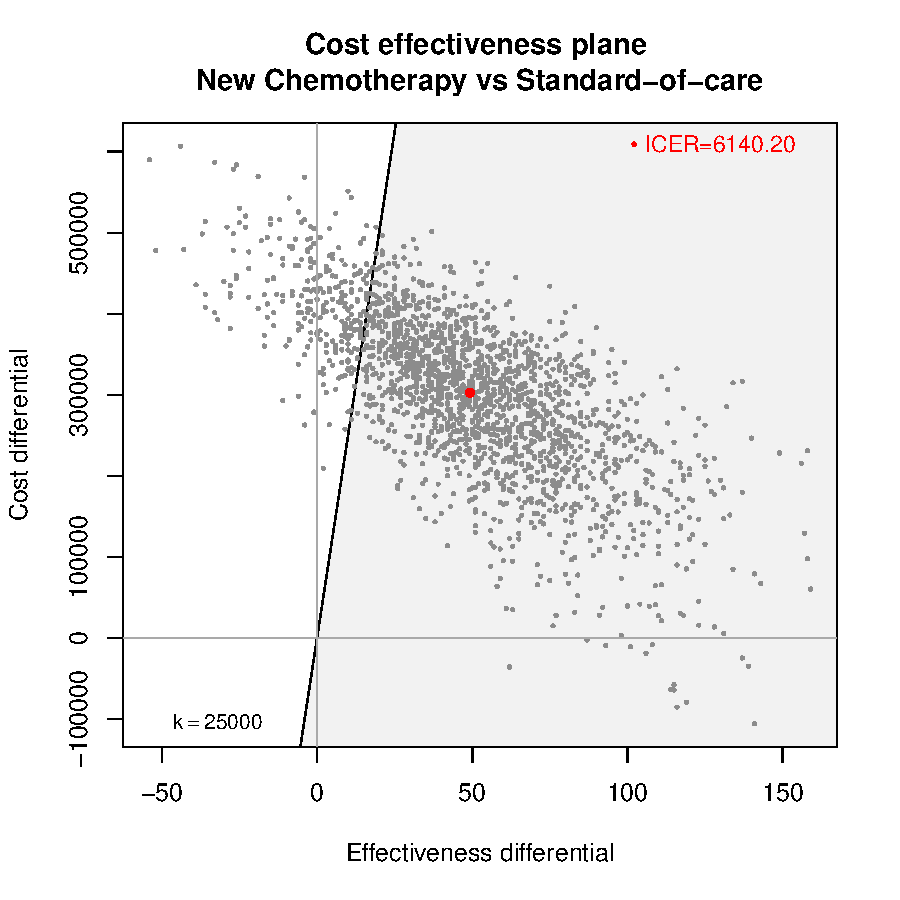
\includegraphics[scale=.5]{6.probabilistic-sensitivity-analysis/figs/chemo_ceplane.pdf}}
\end{center}

\end{frame}

%### New page ############################################################

\begin{frame}

\frametitle{Incremental Cost Effectiveness Ratio (ICER)}

The ICER is the mean incremental cost divided by the mean incremental~effect

\begin{tabular}{ccll}
$\Delta_e$ &$=$& $\mu_2^e - \mu_1^e$ & Expected incremental effects\\
$\Delta_c$ &$=$& $\mu_2^c - \mu_1^c$ & Expected incremental costs
\end{tabular}

\[
\mbox{ICER} = \frac{\mbox{E}[\Delta_c]}{\mbox{E}[\Delta_e]}
\]

\textbf{WARNING!}

\bi
\item The ICER cannot be interpreted without knowing the position of
  $\Delta_e$ and $\Delta_c$ on the CE plane
\item The ICER is not a properly ordered statistic for negative values
  (e.g. -100/100 is better than -100/50 is better than -50/50 in terms
  of decision making, but these ratios are -1, -2, -1)
\ei

\end{frame}

\begin{frame}
\frametitle{Incremental Net (Monetary) Benefit}

{\centering
\fontsize{6.5}{7.5}\selectfont 
\begin{tabular*}{.95\textwidth}{@{\extracolsep{\fill}}lrrrrrrr}
\hline
& \multicolumn{4}{c}{Parameters simulations} & \multicolumn{2}{c}{Expected utility} & \multicolumn{1}{c}{Incremental}  \\
& \multicolumn{2}{c}{$t=0$} & \multicolumn{2}{c}{$t=1$} & \multicolumn{2}{c}{$\mbox{NB}_t(\bm\theta) =k\mu_e-\mu_c$} & \multicolumn{1}{c}{benefit} \\
\cline{2-3} \cline{4-5} \\[-5pt]
Iter/n & \multicolumn{1}{c}{Benefits ($\mu_e$)} & \multicolumn{1}{c}{Costs ($\mu_c$)} & \multicolumn{1}{c}{Benefits ($\mu_e$)} & \multicolumn{1}{c}{Costs ($\mu_c$)} &
\multicolumn{1}{c}{$t=0$} & \multicolumn{1}{c}{$t=1$} & \multicolumn{1}{c}{$k\Delta_e-\Delta_c$} \\
\hline
1 & 741 & 670\,382.1 & 732 & 1\,131\,978 & 19\,214\,751 & 19\,647\,706 &  432\,955.8 \\
2 & 699 & 871\,273.3 & 664 & 1\,325\,654 & 17\,165\,526 & 17\,163\,407 & -2\,119.3 \\
3 & 774 & 639\,071.7 & 706 & 1\,191\,567.2 & 18\,710\,928 & 16\,458\,433 & -2\,252\,495.5 \\
4 & 721 & 1\,033\,679.2 & 792 & 1\,302\,352.2 & 16\,991\,321 & 18\,497\,648 &  1\,506\,327.0 \\
5 & 808 & 427\,101.8 & 784 & 937\,671.1 & 19\,772\,898 & 18\,662\,329 & -1\,110\,569.3 \\
6 & 731 & 1\,168\,864.4 & 811 & 717\,939.2 & 17\,106\,136 & 18\,983\,331 &  1\,877\,195.1 \\
$\ldots$ & \multicolumn{4}{c}{$\ldots$} & \multicolumn{2}{c}{$\ldots$} & $\ldots$ \\
$S$ & 739 & 431\,079.0 & 699 & 1\,004\,195.0 & 18\,043\,921 & 16\,470\,805 & -1\,573\,116.0 \\
\hline
\end{tabular*}
}

\vfill
\begin{itemize}
\item We can analyse the decision-making process ``row-by-row''. Treatment $t=1$ is more cost-effective if 
\[ \myblue \mbox{IB}(\bm\theta) = k\Delta_e - \Delta_c > 0 \]
\item We can plot $\mbox{EIB}=\mbox{E}[\mbox{IB}(\bm\theta)]$ and its 95\% CI for different values of $k$
\item The break-even point occurs at $\mbox{E}[\Delta_{c}]/\mbox{E}[\Delta_{e}]$ 
\begin{itemize}
\item Although it is possible the IB is always positive or negative!
\end{itemize}
\end{itemize}

\end{frame}

%%%%%### New page ############################################################
%%%%
%%%%\begin{frame}
%%%%
%%%%\frametitle{Incremental Net (Monetary) Benefit}
%%%%
%%%%\begin{itemize}
%%%%\item Translate effects onto the cost scale and subtract costs
%%%%
%%%%\item IB($\bm\theta$) = $k\Delta_{e} - \Delta_{c}$ 
%%%%\begin{itemize}
%%%%\item {NB} this is a function of $k$!
%%%%\item $k$ is the amount one is willing to pay for one unit of effectiveness
%%%%\end{itemize}
%%%%
%%%%\item If IB($\bm\theta$)$>$0 then the new treatment is cost effective
%%%%
%%%%\item We can plot the expected IB and its 95\% CI for different values of $k$
%%%%
%%%%\item The break-even point occurs at $\mbox{E}[\Delta_{c}]/\mbox{E}[\Delta_{e}]$ 
%%%%\begin{itemize}
%%%%\item Although it is possible the IB is always positive or negative!
%%%%\end{itemize}
%%%%
%%%%\end{itemize}
%%%%
%%%%\end{frame}

%### New page ############################################################

\begin{frame}

\frametitle{Incremental Net (Monetary) Benefit}

\begin{center}
\rotatebox{0}{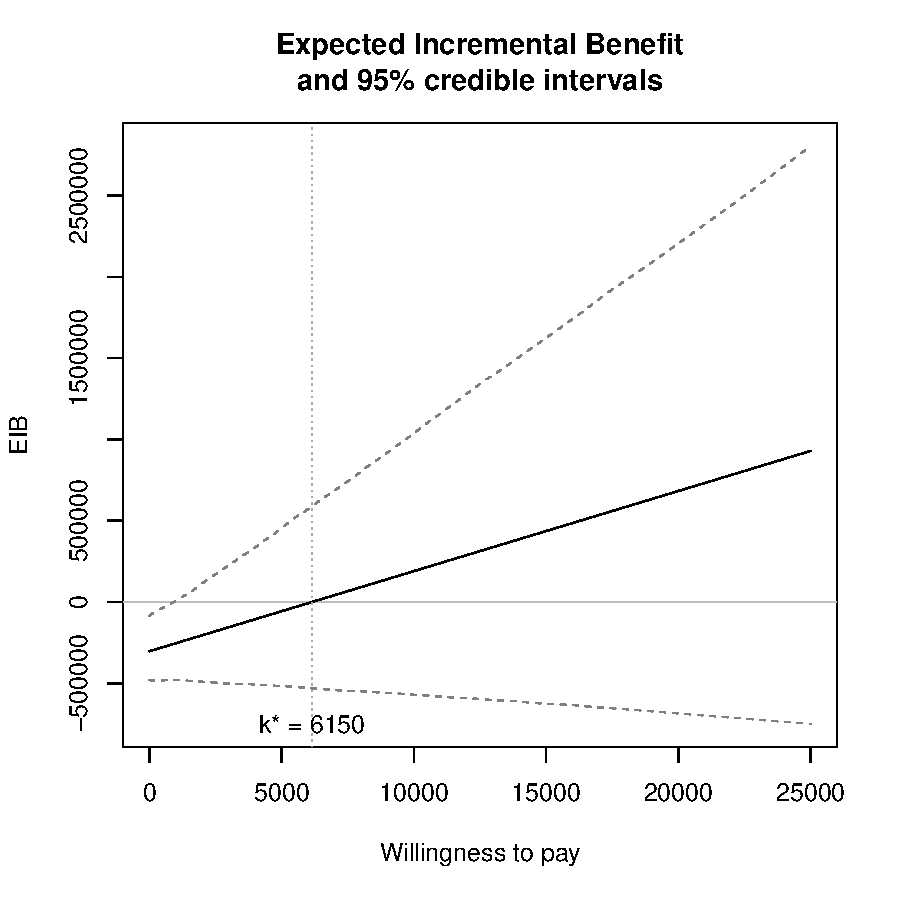
\includegraphics[scale=.53]{6.probabilistic-sensitivity-analysis/figs/chemo_INB.pdf}}
\end{center}

\end{frame}

%### New page ############################################################

\begin{frame}

\frametitle{Cost Effectiveness Acceptability Curve}

\bi
\item To quantify decision uncertainty consider the probability that IB$(\bm\theta)$ is positive

\item $\mbox{CEAC} = \Pr(\mbox{IB}(\bm\theta)>0)=\Pr(k\Delta_{e}-\Delta_{c}>0)$

\item This is the cost-effectiveness acceptability curve (CEAC)

\item Imagine a line on the cost-effectiveness plane going through the origin
and with gradient $k$. The value of CEAC is the area under the line.

\item (Actually CEAC is the volume to one side of a plane bisecting the
probability density function of costs and effects)
\ei

\end{frame}

%% %### New page ############################################################

\begin{frame}

\frametitle{Cost Effectiveness Acceptability Curve}
\vspace{-15pt}
\begin{center}
%\rotatebox{0}{\includegraphics[scale=.53]{chemo_CEAC.pdf}}
\only<1|handout:1>{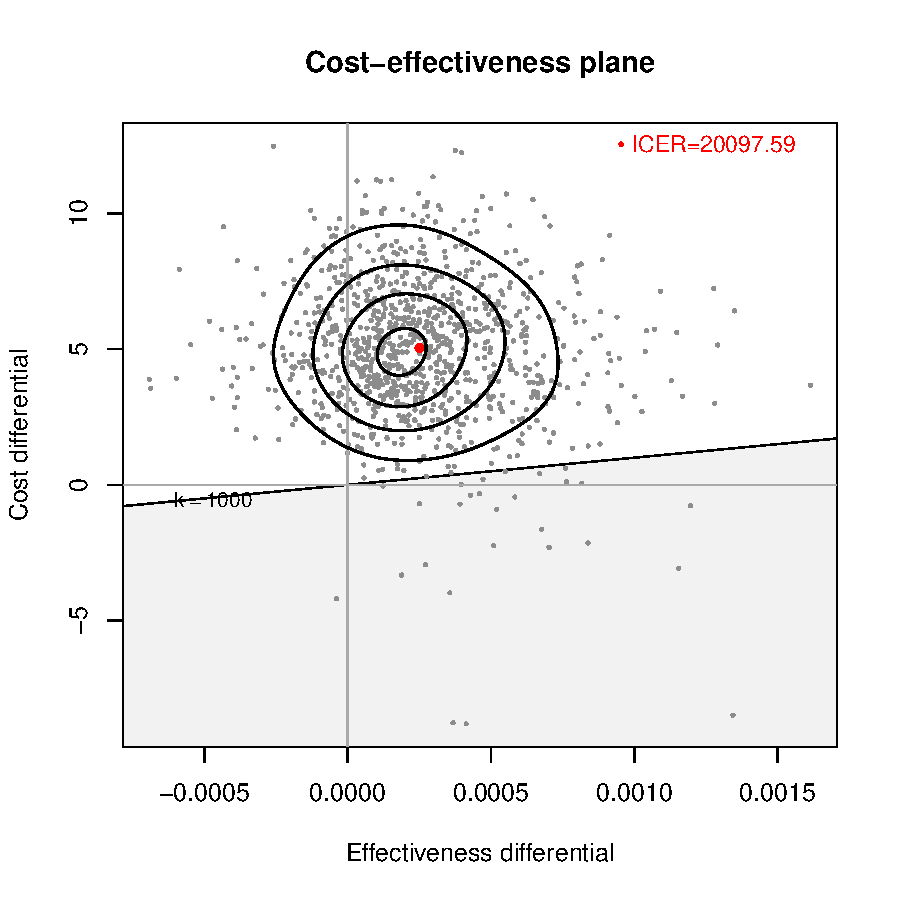
\includegraphics[scale=.53]{6.probabilistic-sensitivity-analysis/figs/CE_plane1}}
\only<2|handout:2>{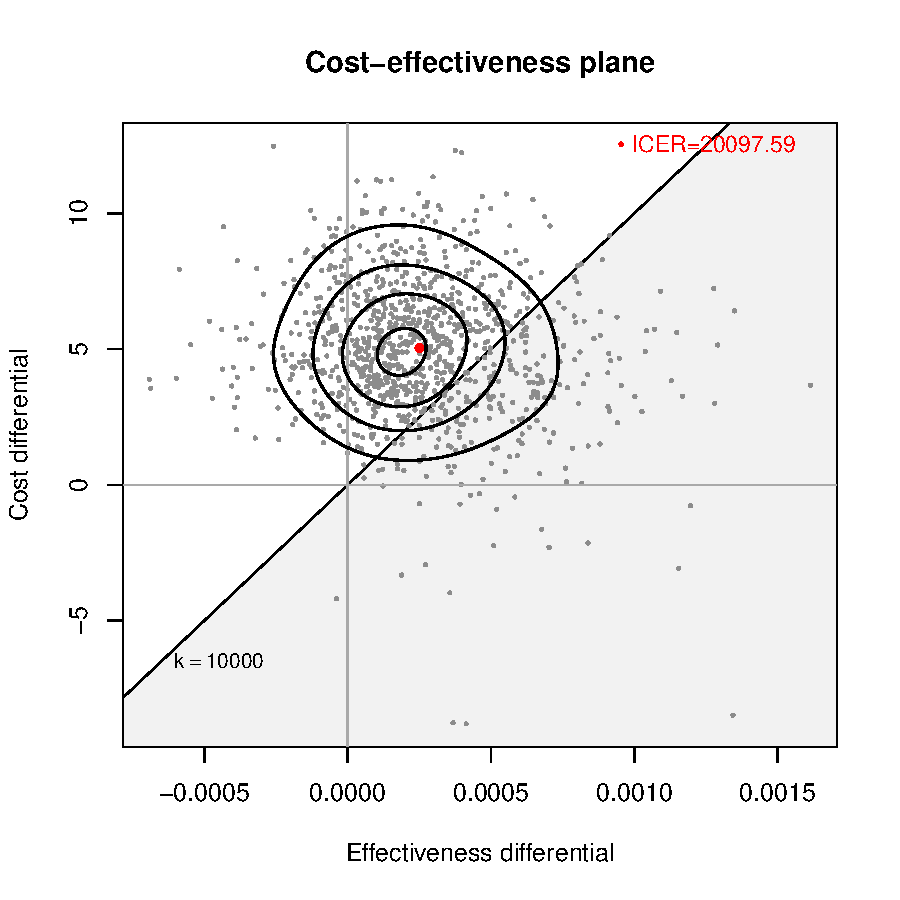
\includegraphics[scale=.53]{6.probabilistic-sensitivity-analysis/figs/CE_plane2}}
\only<3|handout:3>{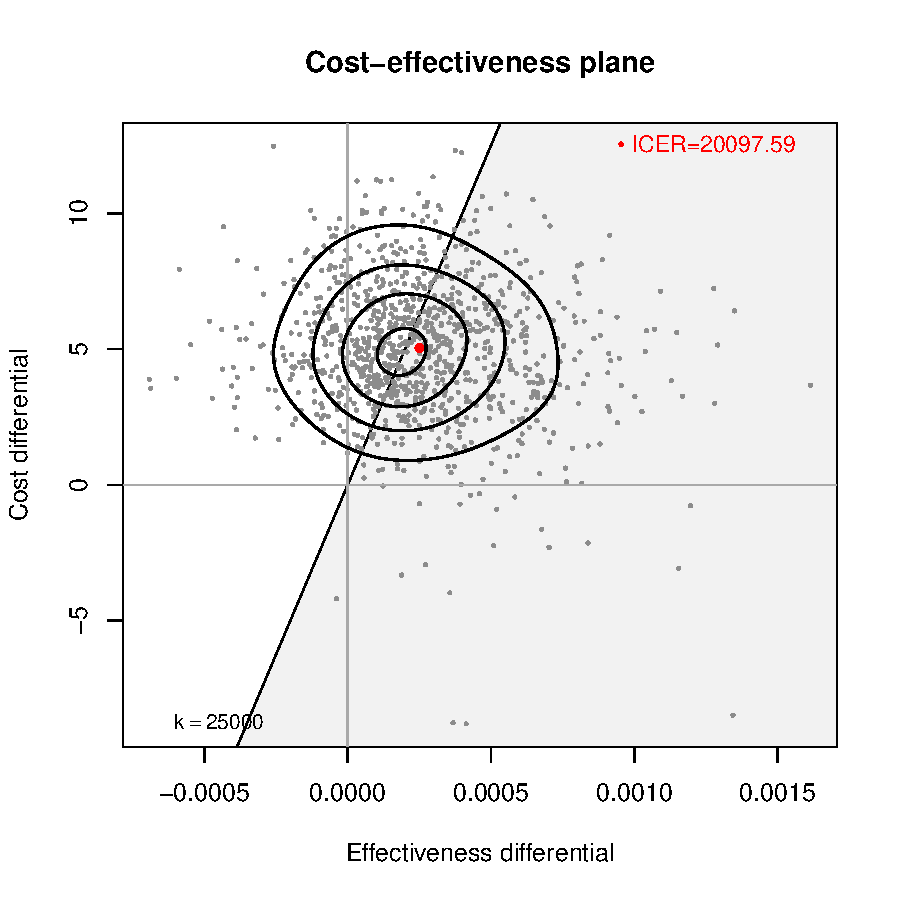
\includegraphics[scale=.53]{6.probabilistic-sensitivity-analysis/figs/CE_plane3}}
\only<4|handout:4>{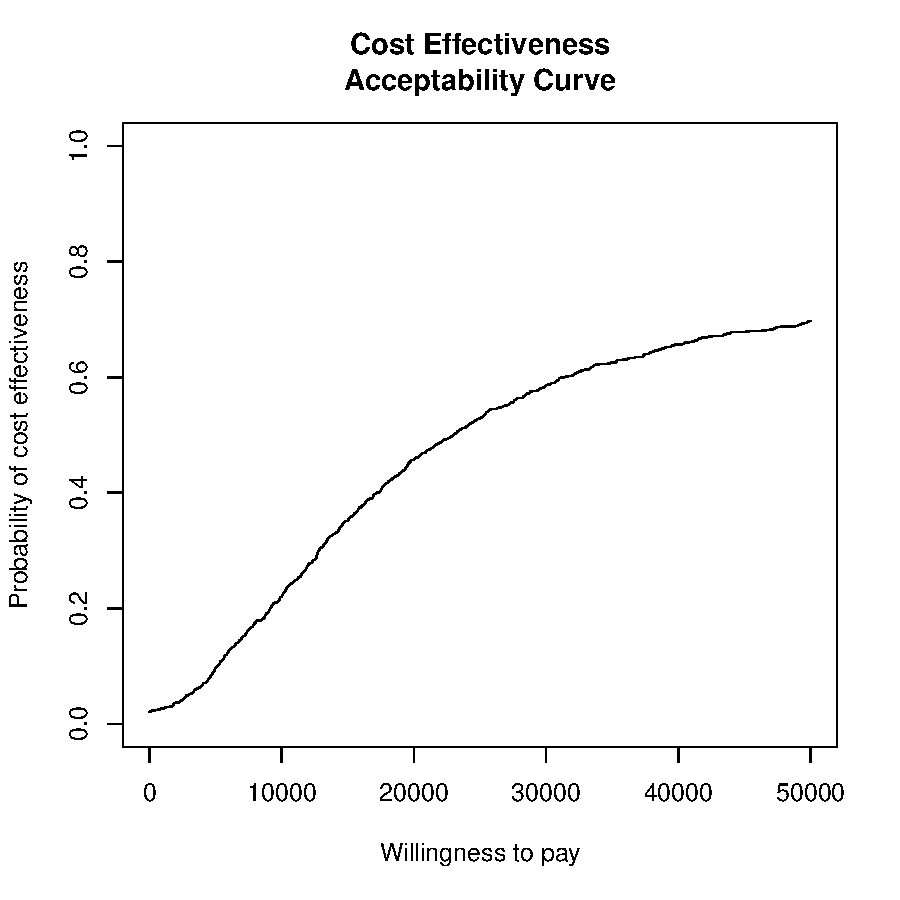
\includegraphics[scale=.53]{6.probabilistic-sensitivity-analysis/figs/CEAC}}
\end{center}
\end{frame}

%% %### New page ############################################################

\begin{frame}[fragile]

\frametitle{Coding this in \bugs}

\begin{verbatim}
## incremental cost/effectiveness ratio
delta.e <- mu.e[2] - mu.e[1]
delta.c <- mu.c[2] - mu.c[1]

##  CEAC curves
k.space <- 5000
for(j in 1:11) {
    k[j]<- (j-1) * k.space
    IB[j] <- k[j] * delta.e - delta.c
    CEAC[j] <- step( IB[j] )
}
\end{verbatim}
\end{frame}

\frame{
\frametitle{Is this \textit{all} we need?}
\begin{itemize}
\item The CEAC only deals with the \textbf{\blue probability} of making the ``right decision''
\item But it does not account for the \textbf{\red payoff/penalty} associated with making the ``wrong'' one!
\vspace{10pt}\pause
\item \textbf{Example 1}: Intervention $t=1$ is the most cost-effective, given current evidence
\begin{itemize}
\item \myblue $\Pr(\mbox{$t=1$ is cost-effective)}=$ 0.51 \black 
\item If we get it wrong: Increase in costs = \pounds 3
\item[] \white If we get it wrong: \black Decrease in effectiveness = 0.000001 QALYs
\item \red Large uncertainty\black/\color{blue!20!black!30!green} negligible consequences \black $\Rightarrow$ \textbf{\color{blue!20!black!30!green}can afford uncertainty}
\end{itemize}
\vspace{5pt}\pause
\item \textbf{Example 2}: Intervention $t=1$ is the most cost-effective, given current evidence
\begin{itemize}
\item \myblue $\Pr(\mbox{$t=1$ is cost-effective)}=$ 0.999 \black 
\item If we get it wrong: Increase in costs = \pounds 1\,000\,000\,000
\item[] \white If we get it wrong: \black Decrease in effectiveness = 999999 QALYs
\item \color{blue!20!black!30!green} Tiny uncertainty\black/\red dire consequences \black $\Rightarrow$ \amber \textbf{probably should think about~it...}
\end{itemize}
\end{itemize}
}

\begin{frame}
\frametitle{Is this \textit{all} we need?}
\hspace{-1cm}\vspace{-1cm}
\begin{figure}
\setcounter{subfigure}{0}
\captionsetup[subfigure]{labelformat=empty}
\begin{center}
\subfloat[\bfseries Example 1]{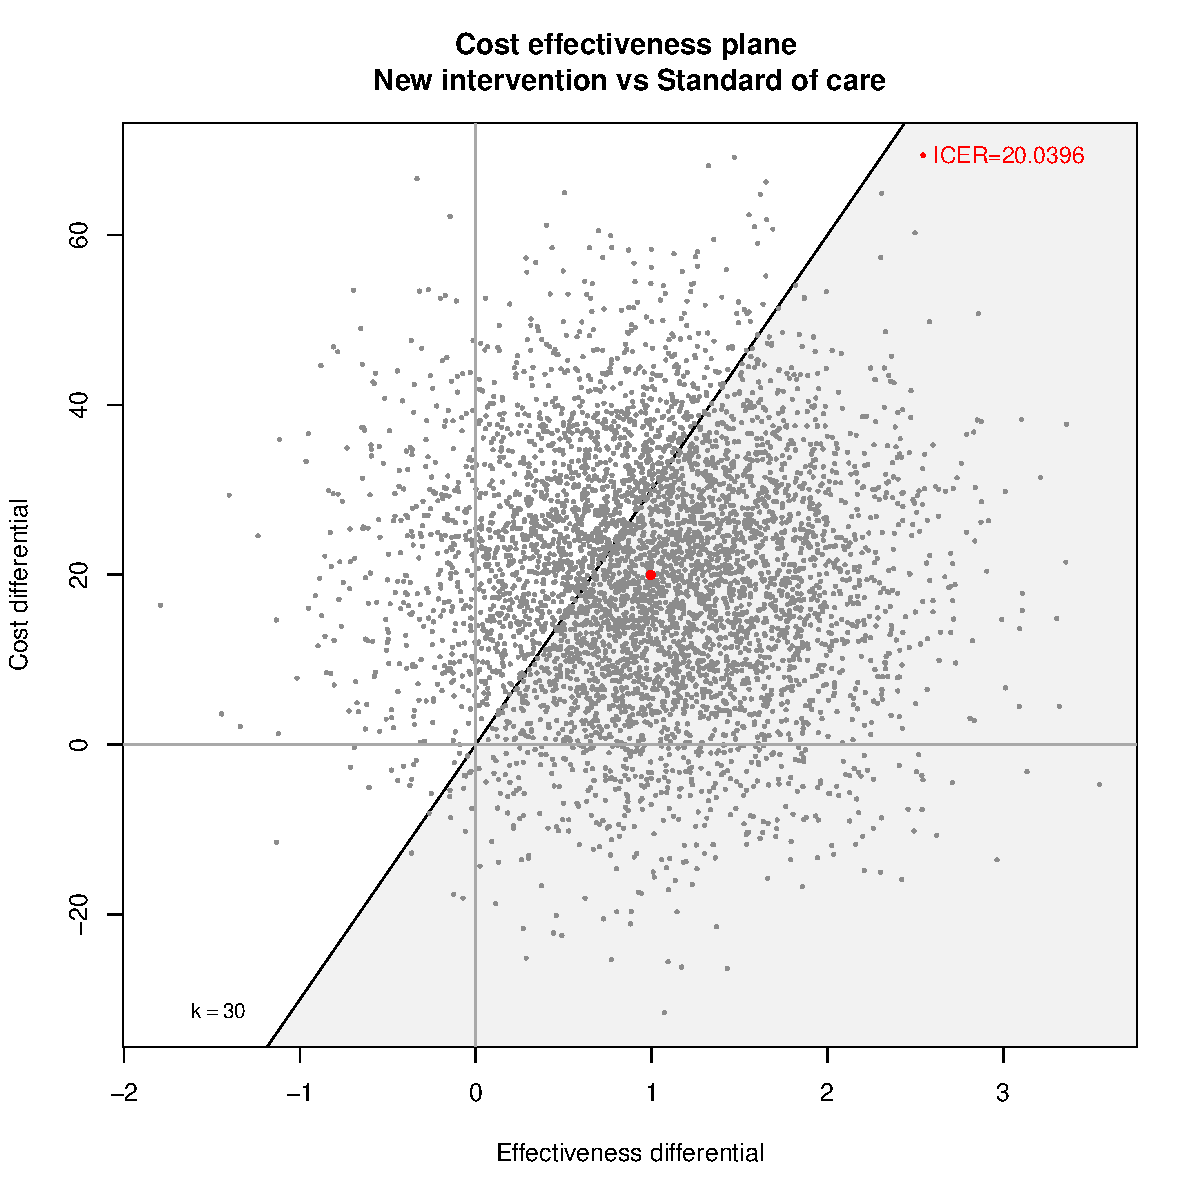
\includegraphics[scale=.28]{6.probabilistic-sensitivity-analysis/figs/CEAC_good}} \hfill
\subfloat[\bfseries Example 2]{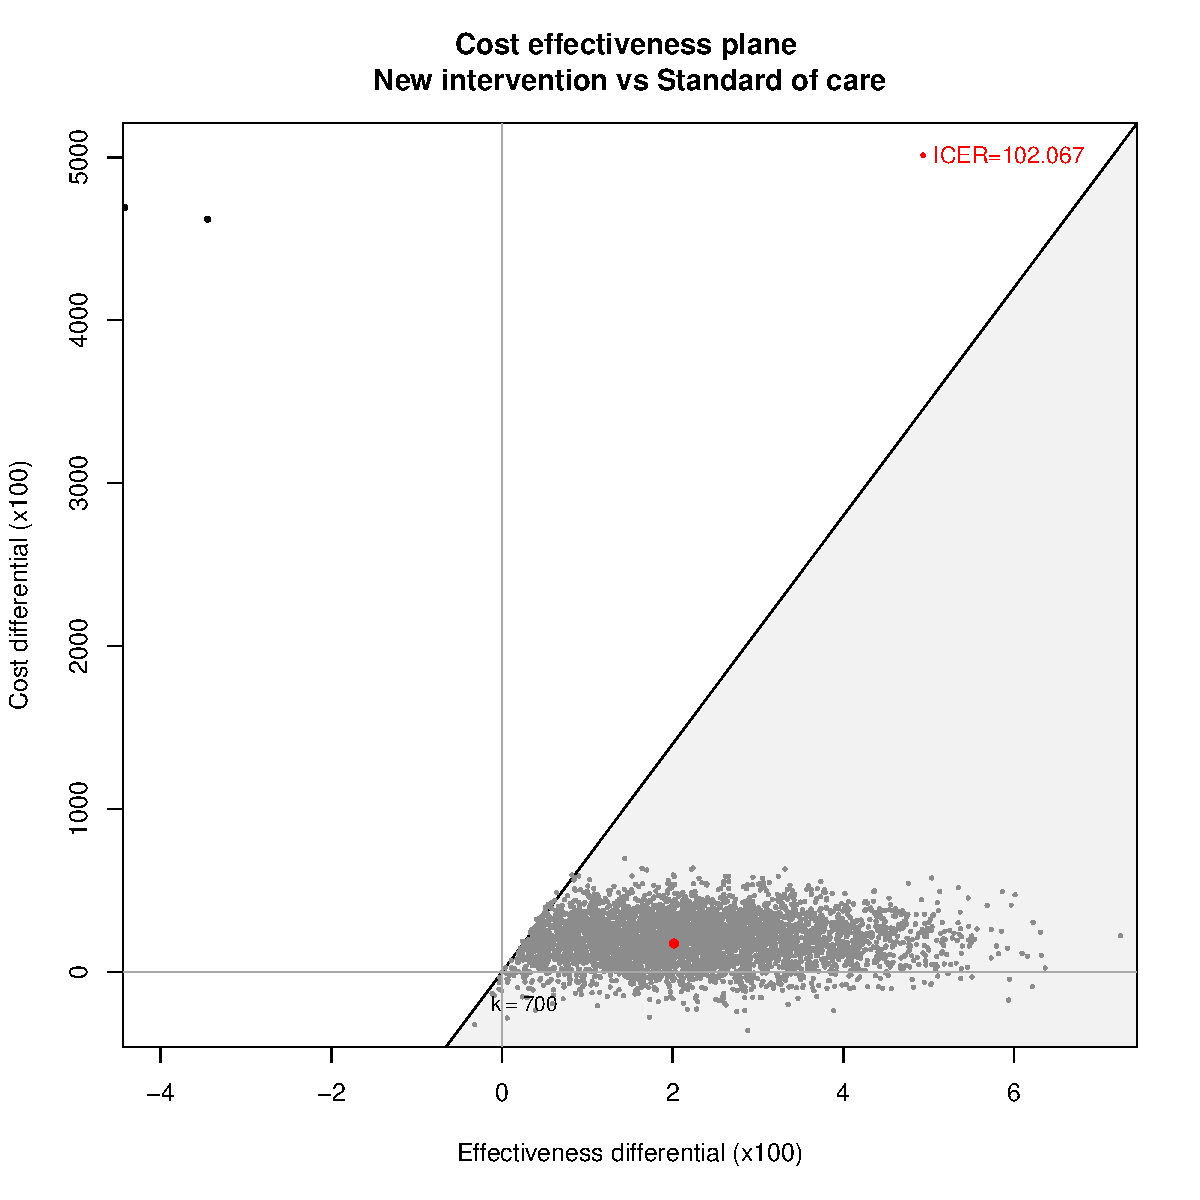
\includegraphics[scale=.28]{6.probabilistic-sensitivity-analysis/figs/CEAC_bad}} 
\end{center}
\end{figure}
\end{frame}

\begin{frame}
\frametitle{Non-identical twins?}
\begin{tabular}{p{5.8cm}p{5.8cm}}
%\begin{tabular}{<{\onslide<2->}p{5.8cm}<{\onslide}p{5.8cm}}
    \begin{minipage}[l]{5.5cm}
   \hspace{-20pt} 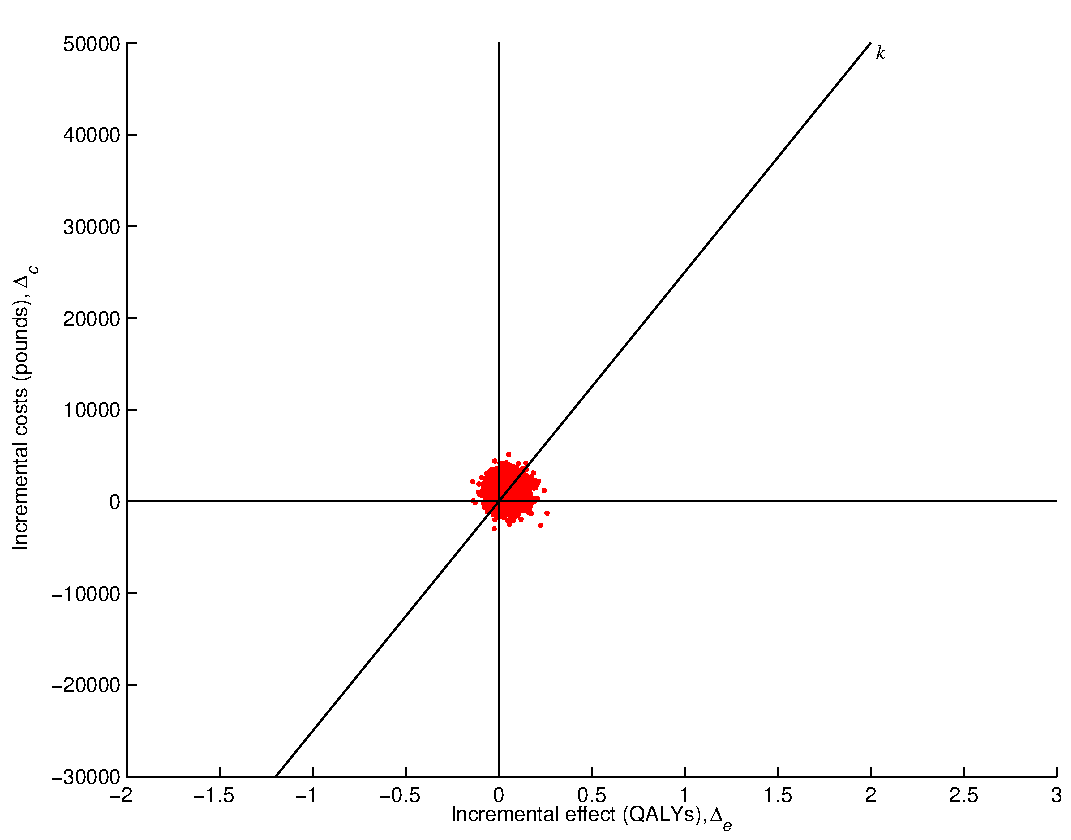
\includegraphics[scale=.35]{6.probabilistic-sensitivity-analysis/figs/ceacLimit1}
    \end{minipage} &
    \begin{minipage}[r]{5.5cm}
    \hspace{-10pt}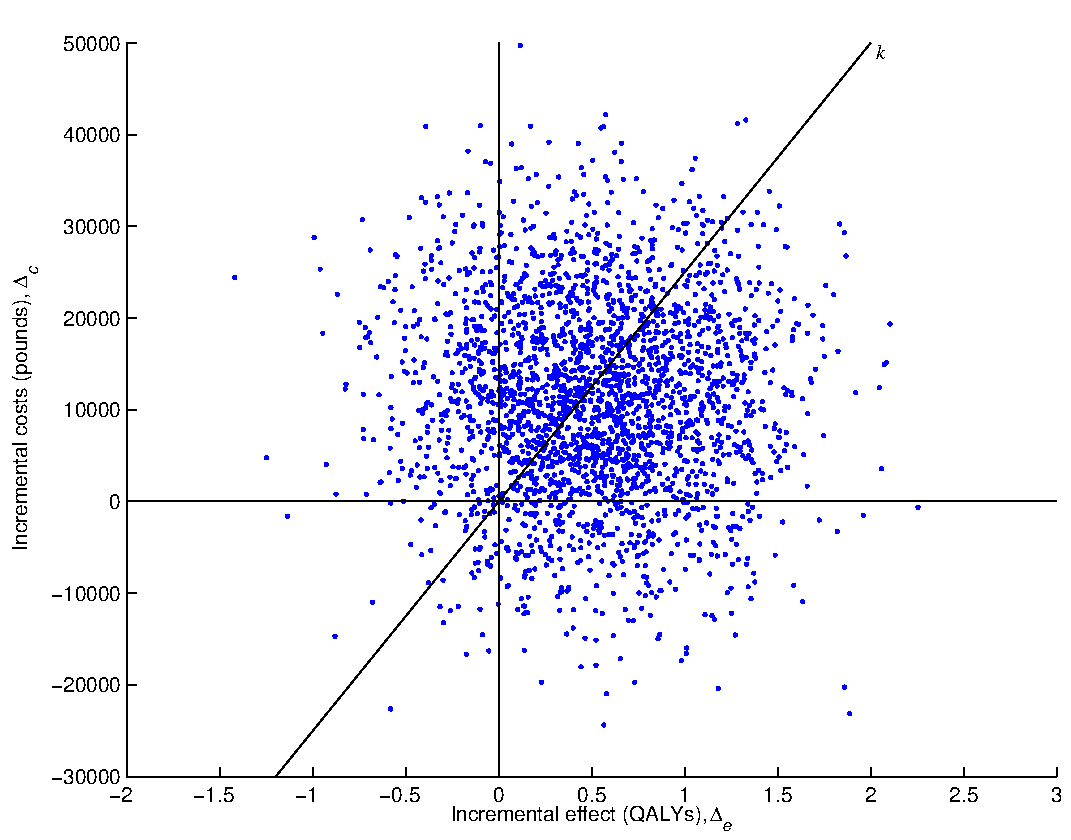
\includegraphics[scale=.35]{6.probabilistic-sensitivity-analysis/figs/ceacLimit2}
    \end{minipage} \\[-5pt]
    \fontsize{8}{8}\selectfont
    \begin{itemize}
        \item $\mbox{E}(\Delta_c)=\textrm{\pounds} 1,100$ \par $\mbox{sd}(\Delta_c)=\textrm{\pounds} 1,100$
        \item $\mbox{E}(\Delta_e)= 0.05$ QALYs \par $\mbox{sd}(\Delta_e)=0.05$ QALYs
        \item $\mbox{Corr}(\Delta_c,\Delta_e)=0$
        \item $\mbox{CEAC} = \Pr\left(k\Delta_e-\Delta_c>0\right)=0.53$ \par per
        $k=\textrm{\pounds}
        25,000$
    \end{itemize}
    &
    \fontsize{8}{8}\selectfont
    \begin{itemize}
        \item $\mbox{E}(\Delta_c)=\textrm{\pounds} 11,000$ \par $\mbox{sd}(\Delta_c)=\textrm{\pounds} 11,000$
        \item $\mbox{E}(\Delta_e)= 0.5$ QALYs \par $\mbox{sd}(\Delta_e)=0.5$ QALYs
        \item $\mbox{Corr}(\Delta_c,\Delta_e)=0$
        \item $\mbox{CEAC} = \Pr\left(k\Delta_e-\Delta_c>0\right)=0.53$ \par per
        $k=\textrm{\pounds}
        25,000$
    \end{itemize}
\end{tabular}
\end{frame}

\frame{
\frametitle{The rationale for PSA / research prioritisation}
\begin{figure}
\begin{tikzpicture}%[->,>=latex,shorten >=0pt,auto,node distance=3cm,ultra thin]
\onslide<1-3|handout:1>{
\node{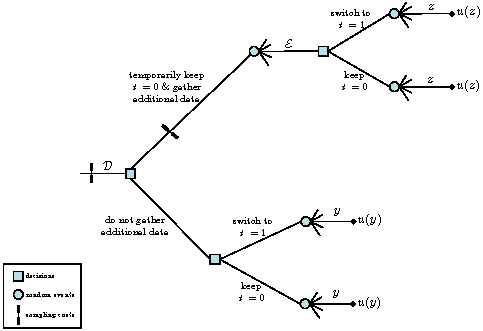
\includegraphics[scale=1.25]{6.probabilistic-sensitivity-analysis/figs/decisionProcess}};
}
\onslide<1|handout:0>{
\draw(-3.3,-.9) node[rectangle,align=center,draw=none,fill=white,text width=5cm,text height=5cm]{};
\draw(-0.3,2) node[rectangle,align=center,draw=none,fill=white,text width=11cm,text height=3cm]{};
}
\onslide<2|handout:0>{
\draw(2.77,2) node[rectangle,align=center,draw=none,fill=white,text width=5cm,text height=3cm]{};
}
\end{tikzpicture}
\end{figure}
}

%%%%%%%%%%%%### New page ############################################################
%%%%%%%%%%%
%%%%%%%%%%%\begin{frame}[fragile]
%%%%%%%%%%%
%%%%%%%%%%%\frametitle{``Push through'' uncertainty}
%%%%%%%%%%%
%%%%%%%%%%%\begin{center}
%%%%%%%%%%%\rotatebox{0}{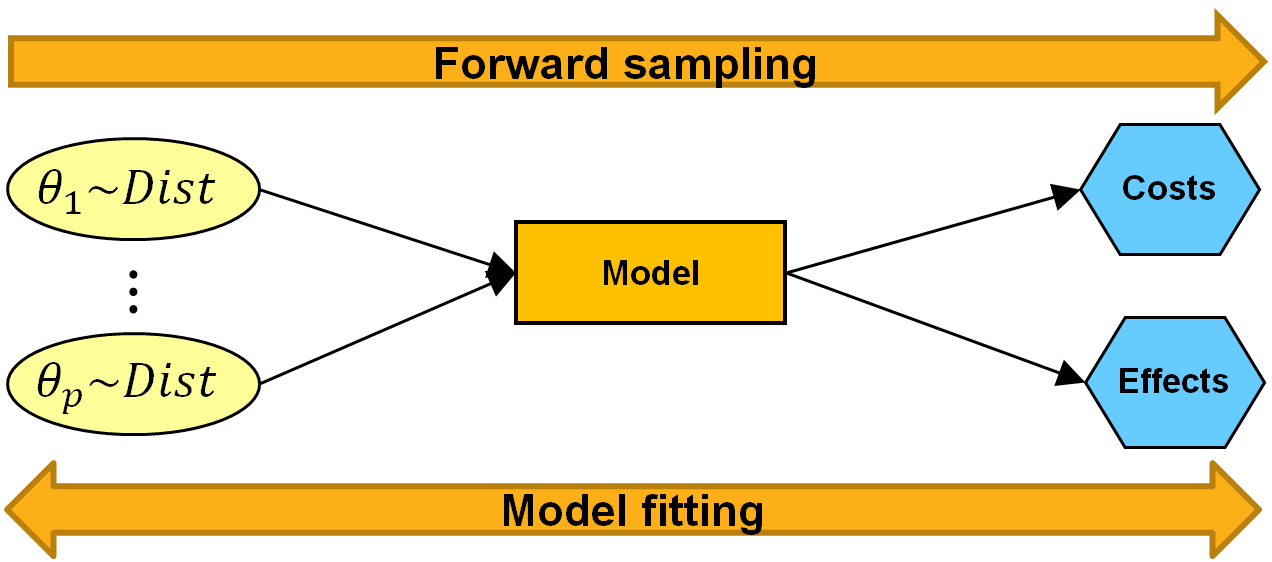
\includegraphics[height=4.5cm]{6.probabilistic-sensitivity-analysis/figs/forward_backward.png}}
%%%%%%%%%%%\end{center}
%%%%%%%%%%%
%%%%%%%%%%%
%%%%%%%%%%%\end{frame}
%%%%%%%%%%%
%%%%%%%%%%%%### New page ############################################################
%%%%%%%%%%%
%%%%%%%%%%%\begin{frame}
%%%%%%%%%%%
%%%%%%%%%%%\frametitle{Summary}
%%%%%%%%%%%
%%%%%%%%%%%\bi
%%%%%%%%%%%
%%%%%%%%%%%\item One step parameter estimation and cost-effectiveness model
%%%%%%%%%%%\bi
%%%%%%%%%%%\item Set up a deterministic health economic model
%%%%%%%%%%%\item Estimate parameters and ``Push through'' the uncertainty in the parameters underpinning this model by Monte Carlo simulation
%%%%%%%%%%%\ei
%%%%%%%%%%%
%%%%%%%%%%%\item  This generates the distribution of the population mean effectiveness and population mean cost in each arm
%%%%%%%%%%%\bi
%%%%%%%%%%%\item $\mathbb{E}[f(\theta)] \neq f\left( \mathbb{E}[\theta] \right) $
%%%%%%%%%%%\ei
%%%%%%%%%%%
%%%%%%%%%%%\item We use these distributions to find
%%%%%%%%%%%\bi
%%%%%%%%%%%\item Incremental cost-effectiveness ratio
%%%%%%%%%%%\item Incremental net benefit
%%%%%%%%%%%\item Cost effectiveness acceptability curves
%%%%%%%%%%%\ei
%%%%%%%%%%%
%%%%%%%%%%%\item We calculate the value of reducing the uncertainty in the parameters
%%%%%%%%%%%\bi
%%%%%%%%%%%\item Expected value of perfect information
%%%%%%%%%%%\item Expected value of perfect partial information
%%%%%%%%%%%\ei
%%%%%%%%%%%\ei
%%%%%%%%%%%
%%%%%%%%%%%%{\footnotesize \emph{Bayesian Methods in Health Economics} chapter 3.4 -- 3.5}
%%%%%%%%%%%
%%%%%%%%%%%\end{frame}
%%%%%%%%%%%
%%%%%%%%%%%
%%%%%%%%%%%%### New page ############################################################
%%%%%%%%%%%
%%%%%%%%%%%\begin{frame}
%%%%%%%%%%%
%%%%%%%%%%%\frametitle{New chemotherapy drug}
%%%%%%%%%%%
%%%%%%%%%%%\bi
%%%%%%%%%%%\item Evaluate a new chemotherapy drug against the standard of care
%%%%%%%%%%%
%%%%%%%%%%%\item Following treatment, a patient may experience haematological side effects
%%%%%%%%%%%
%%%%%%%%%%%\item If this does happen, depending on the severity, the patient either needs ambulatory care, or is admitted to hospital
%%%%%%%%%%%
%%%%%%%%%%%\item Costs to include: Drug costs, cost of ambulatory care, cost of hospital
%%%%%%%%%%%
%%%%%%%%%%%\item Effect: Being free of side effects
%%%%%%%%%%%\ei
%%%%%%%%%%%
%%%%%%%%%%%\end{frame}
%%%%%%%%%%%
%%%%%%%%%%%%### New page ############################################################
%%%%%%%%%%%
%%%%%%%%%%%\begin{frame}
%%%%%%%%%%%
%%%%%%%%%%%\frametitle{Components of Decision Quality\footnote{\fontsize{7}{8}\selectfont Ron Howard. The Foundations of Decision Analysis Revisited, in Advances in Decision Analysis 2007.}}
%%%%%%%%%%%
%%%%%%%%%%%{\footnotesize
%%%%%%%%%%%
%%%%%%%%%%%\bi
%%%%%%%%%%%\item What we can do?
%%%%%%%%%%%\bi
%%%%%%%%%%%\item $t$ is the set of interventions
%%%%%%%%%%%\item Decide to use standard-or-care or new treatment ($t = 1, 2$)
%%%%%%%%%%%\ei
%%%%%%%%%%%
%%%%%%%%%%%\item What we know?
%%%%%%%%%%%\bi
%%%%%%%%%%%\item Statistically these are the \alert{random variables}
%%%%%%%%%%%\item $\mathbf{\theta}$: parameters describing  disease model, costs and effects
%%%%%%%%%%%\item $e$ and $c$ are the observable outcomes
%%%%%%%%%%%\item $\mu_t^e = \mathbb{E}[e\mid\theta, t]$ and $\mu_t^c= \mathbb{E}[c\mid\theta, t]$ are population mean cost and effect given intervention $t$.
%%%%%%%%%%%\ei
%%%%%%%%%%%
%%%%%%%%%%%\item What we want?
%%%%%%%%%%%\bi
%%%%%%%%%%%\item The value of the outcomes \alert{measured by utility}
%%%%%%%%%%%\item We chose the \alert{net (monetary) benefit}\\
%%%%%%%%%%%$u(e,c;t) = ke-c$\\
%%%%%%%%%%%$k$ is the willingness-to-pay for one unit of effectivness.
%%%%%%%%%%%\item Chose intervention $t$ with the highest expected net benefit\\
%%%%%%%%%%%$\mathbb{E}\left[ \mathbb{E}[u(e,c;t)] \right] = \mathbb{E}\left[k\mu_t^e-\mu_t^c \right]$\\
%%%%%%%%%%%\ei
%%%%%%%%%%%\ei
%%%%%%%%%%%
%%%%%%%%%%%}
%%%%%%%%%%%
%%%%%%%%%%%\end{frame}
%%%%%%%%%%%
%%%%%%%%%%%%### New page ############################################################
%%%%%%%%%%%
%%%%%%%%%%%\begin{frame}
%%%%%%%%%%%
%%%%%%%%%%%\frametitle{Decision tree model}
%%%%%%%%%%%
%%%%%%%%%%%
%%%%%%%%%%%\begin{center}
%%%%%%%%%%%\rotatebox{0}{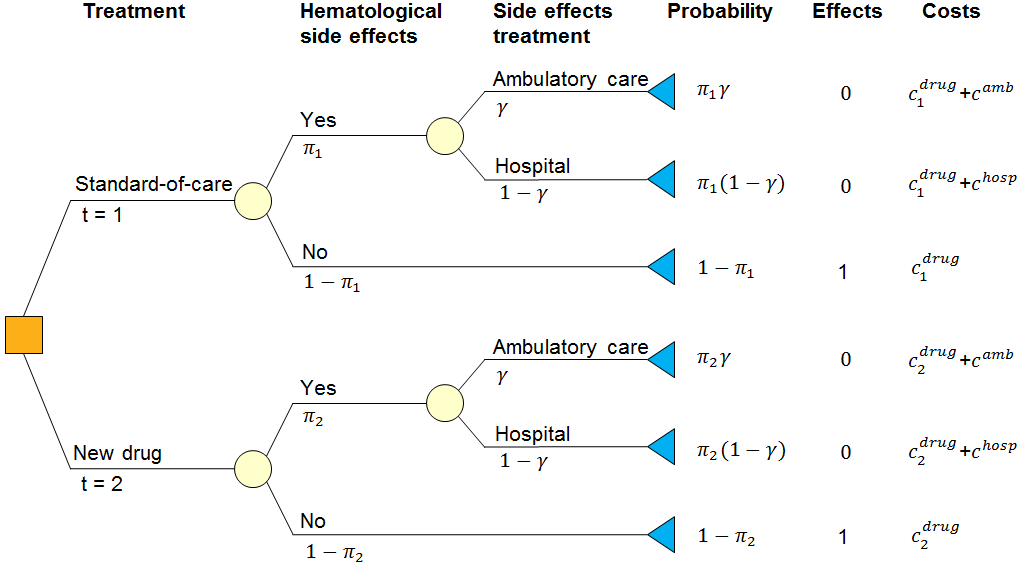
\includegraphics[height=6.5cm]{6.probabilistic-sensitivity-analysis/figs/chemo_decision_tree.png}}
%%%%%%%%%%%\end{center}
%%%%%%%%%%%
%%%%%%%%%%%
%%%%%%%%%%%\end{frame}
%%%%%%%%%%%
%%%%%%%%%%%%### New page ############################################################
%%%%%%%%%%%
%%%%%%%%%%%\begin{frame}
%%%%%%%%%%%
%%%%%%%%%%%\frametitle{Disease model data}
%%%%%%%%%%%
%%%%%%%%%%%We have data from a clinical study
%%%%%%%%%%%
%%%%%%%%%%%
%%%%%%%%%%%\begin{center}
%%%%%%%%%%%\small
%%%%%%%%%%%\begin{tabular}{lrl}
%%%%%%%%%%%\hline
%%%%%%%%%%%Parameter  & Value & Description\\
%%%%%%%%%%%\hline
%%%%%%%%%%%$N^{pat}$ & 111 & Number of patients in observed data \\
%%%%%%%%%%%$N^{se}$  & 27  & Number of patients with side effects,  \\ &&given standard-of-care \\
%%%%%%%%%%%$N^{amb}$ & 17  & Number of patient with ambulatory care following \\ &&side effect, given standard-of-care \\
%%%%%%%%%%%$\mu_{\rho}$ & 0.8  & Mean relative probability of side effects \\ &&in new treatment compared to standard-of-care \\
%%%%%%%%%%%$\sigma_{\rho}$ & 0.2  & SE of relative probability of side effects \\ &&in new treatment compared to standard-of-care \\
%%%%%%%%%%%\hline
%%%%%%%%%%%
%%%%%%%%%%%\end{tabular}
%%%%%%%%%%%\end{center}
%%%%%%%%%%%
%%%%%%%%%%%
%%%%%%%%%%%\end{frame}
%%%%%%%%%%%
%%%%%%%%%%%%### New page ############################################################
%%%%%%%%%%%
%%%%%%%%%%%\begin{frame}[fragile]
%%%%%%%%%%%
%%%%%%%%%%%\frametitle{Disease model analysis}
%%%%%%%%%%%
%%%%%%%%%%%{\small
%%%%%%%%%%%Probability of side effects
%%%%%%%%%%%
%%%%%%%%%%%\begin{tabular}{ccll}
%%%%%%%%%%%$N^{\rm{se}}$ & $\sim$ & ${\rm Binomial}(\pi_1, N^{\rm{pat}})$         & sampling distribution \\
%%%%%%%%%%%$\pi_1$           & $\sim$ & ${\rm Beta}(1, 1)$                                & prior distribution \\
%%%%%%%%%%%$\rho$            & $\sim$ & ${\rm Normal}(\mu_{\rho}, \sigma_{\rho}^2)$ & Reduction in the occurence of side effects \\
%%%%%%%%%%%$\pi_2$           & $=$    & $\rho \pi_1$                                      &  \\
%%%%%%%%%%%\end{tabular}
%%%%%%%%%%%
%%%%%%%%%%%Treatment of side effects
%%%%%%%%%%%
%%%%%%%%%%%\begin{tabular}{ccll}
%%%%%%%%%%%$N^{\rm{amb}}$ & $\sim$  & ${\rm Binomial}(\gamma, N^{\rm{se}})$  & sampling distribution \\
%%%%%%%%%%%$\mathtt{\gamma}$  &  $\sim$ & ${\rm Beta}(1, 1)$                         & prior distribution \\
%%%%%%%%%%%\end{tabular}
%%%%%%%%%%%
%%%%%%%%%%%\begin{verbatim}
%%%%%%%%%%%num.se ~ dbin(pi[1], num.pat)
%%%%%%%%%%%pi[1] ~ dbeta(1, 1)
%%%%%%%%%%%
%%%%%%%%%%%rho ~ dnorm(m.rho, tau.rho)
%%%%%%%%%%%pi[2] <- rho * pi[1]
%%%%%%%%%%%
%%%%%%%%%%%num.amb ~ dbin(gamma, num.se)
%%%%%%%%%%%gamma ~ dbeta(1, 1)
%%%%%%%%%%%
%%%%%%%%%%%\end{verbatim}
%%%%%%%%%%%}
%%%%%%%%%%%
%%%%%%%%%%%\end{frame}
%%%%%%%%%%%
%%%%%%%%%%%
%%%%%%%%%%%%### New page ############################################################
%%%%%%%%%%%
%%%%%%%%%%%\begin{frame}[fragile]
%%%%%%%%%%%
%%%%%%%%%%%\frametitle{Cost Data}
%%%%%%%%%%%
%%%%%%%%%%%{\footnotesize
%%%%%%%%%%%\begin{center}
%%%%%%%%%%%\begin{tabular}{lrll}
%%%%%%%%%%%\hline
%%%%%%%%%%%Parameter  & Distribution & Description & Mean cost\\
%%%%%%%%%%%  \hline\\[-6pt]
%%%%%%%%%%%  $c^{\rm{amb}}$ & logNormal(4.77, 0.17) & Ambulatory care & 120 \\
%%%%%%%%%%%  $c^{\rm{hosp}}$ &  logNormal(8.60, 0.18) & Hospital & 5483 \\
%%%%%%%%%%%  $c_1^{\rm{drug}}$ & 110  & Cost of standard-of-care \\
%%%%%%%%%%%  $c_2^{\rm{drug}}$ & 520 & Cost of new drug \\
%%%%%%%%%%%  \hline
%%%%%%%%%%%\end{tabular}
%%%%%%%%%%%\end{center}
%%%%%%%%%%%}
%%%%%%%%%%%
%%%%%%%%%%%{\small
%%%%%%%%%%%\begin{verbatim}
%%%%%%%%%%%c.amb ~ dlnorm(m.amb, tau.amb)     # Cost of ambulatory care
%%%%%%%%%%%c.hosp ~ dlnorm(m.hosp, tau.hosp)  # Cost of hospitalization
%%%%%%%%%%%
%%%%%%%%%%%# The drug costs are part of the data set
%%%%%%%%%%%list(c.drug = c(110, 520))
%%%%%%%%%%%\end{verbatim}
%%%%%%%%%%%}
%%%%%%%%%%%
%%%%%%%%%%%\end{frame}
%%%%%%%%%%%
%%%%%%%%%%%
%%%%%%%%%%%%### New page ############################################################
%%%%%%%%%%%
%%%%%%%%%%%\begin{frame}[fragile]
%%%%%%%%%%%\frametitle{The predictive distributions and total costs and effects}
%%%%%%%%%%%
%%%%%%%%%%%{\footnotesize
%%%%%%%%%%%\begin{tabular}{ccll}
%%%%%%%%%%%$N$     & $=$ & \multicolumn{2}{l}{Number of patients in the population to model} \\
%%%%%%%%%%%$SE_t$  & $\sim$ & ${\rm Binomial}(\pi_t, N)$            & Expected \#  with side effects \\
%%%%%%%%%%%$A_t$   & $\sim$ & ${\rm Binomial}(\lambda, SE_t)$          & Expected \#  with with ambulatory care\\
%%%%%%%%%%%$H_t$   & $=$ & $SE_t - A_t$                           & Expected \# with with hospitalization \\
%%%%%%%%%%%$\mu_t^e$  & $=$ & $ N - SE_t$                   & Expected \# with no side effects \\
%%%%%%%%%%%$\mu_t^c$  & $=$ & $ c_t^{\rm{drug}} N + c^{\rm{amb}} A_t +c^{\rm{hosp}} H_t$ & Expected cost \\
%%%%%%%%%%%\end{tabular}
%%%%%%%%%%%}
%%%%%%%%%%%
%%%%%%%%%%%{\small
%%%%%%%%%%%\begin{verbatim}
%%%%%%%%%%%for (t in 1:2){
%%%%%%%%%%%    SE[t] ~ dbin(pi[t], N)
%%%%%%%%%%%    A[t] ~ dbin(gamma, SE[t])
%%%%%%%%%%%    H[t] <- SE[t] - A[t]
%%%%%%%%%%%    mu.e[t] <- N - SE[t]
%%%%%%%%%%%    mu.c[t] <- c.drug[t] * N + c.amb * A[t] + c.hosp * H[t]
%%%%%%%%%%%}
%%%%%%%%%%%\end{verbatim}
%%%%%%%%%%%}
%%%%%%%%%%%
%%%%%%%%%%%\end{frame}
%%%%%%%%%%%
%%%%%%%%%%%%### New page ############################################################
%%%%%%%%%%%
%%%%%%%%%%%\begin{frame}
%%%%%%%%%%%
%%%%%%%%%%%\frametitle{Cost-effectiveness plane}
%%%%%%%%%%%
%%%%%%%%%%%\begin{center}
%%%%%%%%%%%\rotatebox{0}{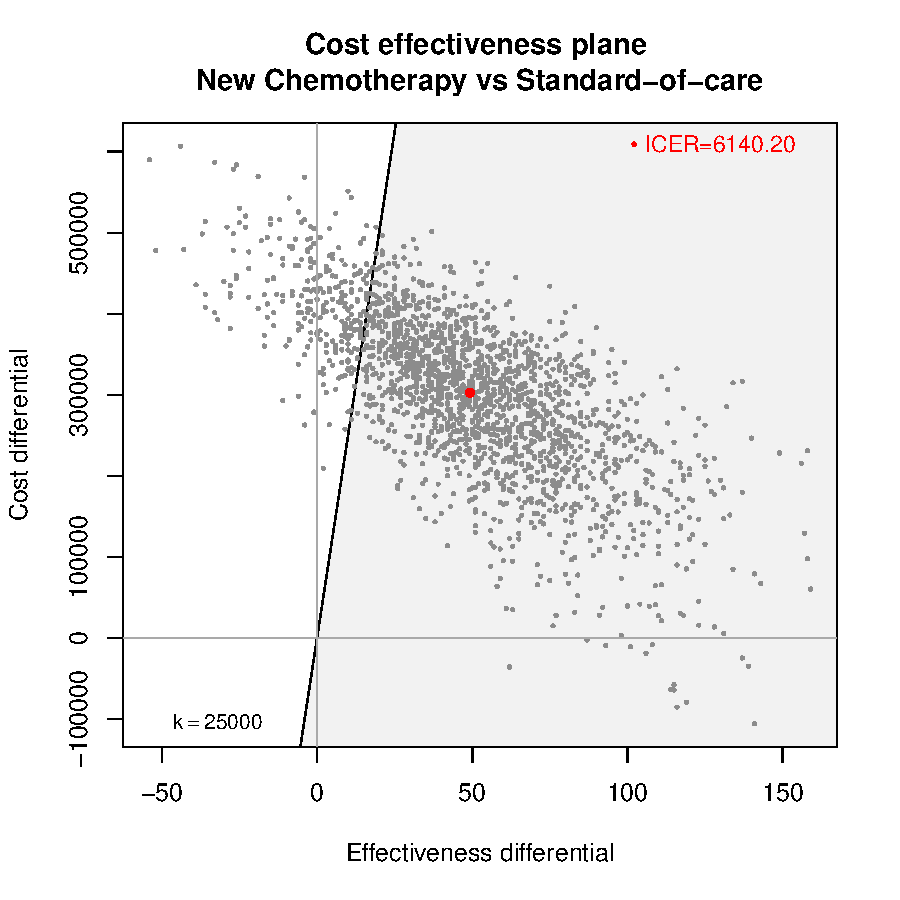
\includegraphics[height=6cm]{6.probabilistic-sensitivity-analysis/figs/chemo_ceplane.pdf}}
%%%%%%%%%%%\end{center}
%%%%%%%%%%%
%%%%%%%%%%%k is the amount one is willing to pay for one unit of effectiveness
%%%%%%%%%%%\end{frame}
%%%%%%%%%%%
%%%%%%%%%%%%### New page ############################################################
%%%%%%%%%%%
%%%%%%%%%%%\begin{frame}
%%%%%%%%%%%
%%%%%%%%%%%\frametitle{Incremental Cost Effectiveness Ratio (ICER)}
%%%%%%%%%%%
%%%%%%%%%%%The ICER is the mean incremental cost divided by the mean incremental effect
%%%%%%%%%%%
%%%%%%%%%%%\begin{tabular}{ccll}
%%%%%%%%%%%$\Delta_e$ &$=$& $\mu_2^e - \mu_1^e$ & Expected incremental effects\\
%%%%%%%%%%%$\Delta_c$ &$=$& $\mu_2^c - \mu_1^c$ & Expected incremental costs
%%%%%%%%%%%\end{tabular}
%%%%%%%%%%%
%%%%%%%%%%%\[
%%%%%%%%%%%\mathrm{ICER} = \frac{\mathbb{E}[\Delta_c]}{\mathbb{E}[\Delta_e]}
%%%%%%%%%%%\]
%%%%%%%%%%%
%%%%%%%%%%%WARNING!
%%%%%%%%%%%
%%%%%%%%%%%\bi
%%%%%%%%%%%\item The ICER cannot be interpreted without knowing the position of
%%%%%%%%%%%  $\Delta_e$ and $\Delta_c$ on the CE plane
%%%%%%%%%%%\item The ICER is not a properly ordered statistic for negative values
%%%%%%%%%%%  (e.g. -100/100 is better than -100/50 is better than -50/50 in terms
%%%%%%%%%%%  of decision making, but these ratios are -1, -2, -1)
%%%%%%%%%%%\ei
%%%%%%%%%%%
%%%%%%%%%%%\end{frame}
%%%%%%%%%%%
%%%%%%%%%%%%### New page ############################################################
%%%%%%%%%%%
%%%%%%%%%%%\begin{frame}
%%%%%%%%%%%
%%%%%%%%%%%\frametitle{Incremental Net (Monetary) Benefit}
%%%%%%%%%%%
%%%%%%%%%%%\begin{itemize}
%%%%%%%%%%%\item Translate effects onto the cost scale and subtract costs
%%%%%%%%%%%
%%%%%%%%%%%\item INB($\theta, k$) = $	k\Delta_{e} - \Delta_{c}$
%%%%%%%%%%%
%%%%%%%%%%%\item $k$ is the amount one is willing to pay for one unit of effectiveness
%%%%%%%%%%%
%%%%%%%%%%%\item If INB($\theta$, k)$>$0 then the new treatment is cost effective
%%%%%%%%%%%
%%%%%%%%%%%\item We can plot the expected INB and its 95\% CI for different values of $k$
%%%%%%%%%%%
%%%%%%%%%%%\item The break-even point occurs at $\mathbb{E}[\Delta_{c}]/\mathbb{E}[\Delta_{e}]$. (Although it is possible the INB is always positive or negative)
%%%%%%%%%%%
%%%%%%%%%%%\end{itemize}
%%%%%%%%%%%
%%%%%%%%%%%\end{frame}
%%%%%%%%%%%
%%%%%%%%%%%%### New page ############################################################
%%%%%%%%%%%
%%%%%%%%%%%\begin{frame}
%%%%%%%%%%%
%%%%%%%%%%%\frametitle{Incremental Net (Monetary) Benefit}
%%%%%%%%%%%
%%%%%%%%%%%\begin{center}
%%%%%%%%%%%\rotatebox{0}{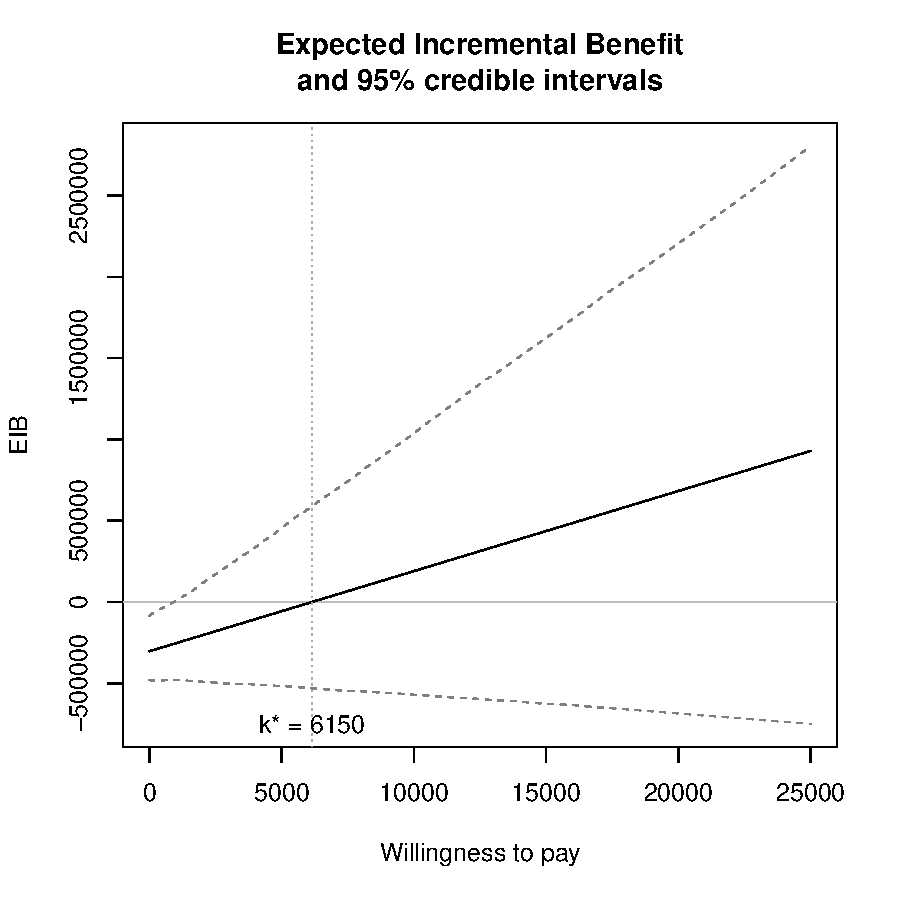
\includegraphics[height=7cm]{6.probabilistic-sensitivity-analysis/figs/chemo_INB.pdf}}
%%%%%%%%%%%\end{center}
%%%%%%%%%%%
%%%%%%%%%%%\end{frame}
%%%%%%%%%%%
%%%%%%%%%%%%### New page ############################################################
%%%%%%%%%%%
%%%%%%%%%%%\begin{frame}
%%%%%%%%%%%
%%%%%%%%%%%\frametitle{Cost Effectiveness Acceptability Curve}
%%%%%%%%%%%
%%%%%%%%%%%\bi
%%%%%%%%%%%\item To quantify decision uncertainty consider the probability that INB(K) is positive
%%%%%%%%%%%
%%%%%%%%%%%\item $Q(k) = \Pr(INB(k)>0)=\Pr(k\Delta_{e}-\Delta_{c}>0)$
%%%%%%%%%%%
%%%%%%%%%%%\item This is the cost-effectiveness acceptability curve (CEAC)
%%%%%%%%%%%
%%%%%%%%%%%\item Imagine a line on the cost-effectiveness plane going through the origin
%%%%%%%%%%%and with gradient $k$. The value of $Q(k)$ is the area under the line.
%%%%%%%%%%%
%%%%%%%%%%%\item (Actually $Q(k)$ is the volume to one side of a plane bisecting the
%%%%%%%%%%%probability density function of costs and effects)
%%%%%%%%%%%\ei
%%%%%%%%%%%
%%%%%%%%%%%\end{frame}
%%%%%%%%%%%
%%%%%%%%%%%%% %### New page ############################################################
%%%%%%%%%%%
%%%%%%%%%%%\begin{frame}
%%%%%%%%%%%
%%%%%%%%%%%\frametitle{Cost Effectiveness Acceptability Curve}
%%%%%%%%%%%
%%%%%%%%%%%\begin{center}
%%%%%%%%%%%\rotatebox{0}{\includegraphics[height=7cm]{6.probabilistic-sensitivity-analysis/figs/chemo_CEAC.pdf}}
%%%%%%%%%%%\end{center}
%%%%%%%%%%%
%%%%%%%%%%%
%%%%%%%%%%%\end{frame}
%%%%%%%%%%%
%%%%%%%%%%%%% %### New page ############################################################
%%%%%%%%%%%
%%%%%%%%%%%\begin{frame}[fragile]
%%%%%%%%%%%
%%%%%%%%%%%\frametitle{Coding this in \bugs}
%%%%%%%%%%%
%%%%%%%%%%%\begin{verbatim}
%%%%%%%%%%%## incremental cost/effectiveness ratio
%%%%%%%%%%%delta.e <- mu.e[2] - mu.e[1]
%%%%%%%%%%%delta.c <- mu.c[2] - mu.c[1]
%%%%%%%%%%%
%%%%%%%%%%%##  CEAC curves
%%%%%%%%%%%k.space <- 5000
%%%%%%%%%%%for(j in 1:11){
%%%%%%%%%%%    k[j]<- (j-1) * k.space
%%%%%%%%%%%    INB[j] <- k[j] * delta.e - delta.c
%%%%%%%%%%%    Q[j] <- step( INB[j] )
%%%%%%%%%%%}
%%%%%%%%%%%\end{verbatim}
%%%%%%%%%%%
%%%%%%%%%%%\end{frame}
%%%%%%%%%%%
%%%%%%%%%%%%### New page ############################################################
%%%%%%%%%%%
%%%%%%%%%%%\begin{frame}
%%%%%%%%%%%
%%%%%%%%%%%\frametitle{Value of perfect information (VPI)}
%%%%%%%%%%%
%%%%%%%%%%%\bi
%%%%%%%%%%%\item Consider a simpler model where:
%%%%%%%%%%%    \bi
%%%%%%%%%%%    \item The only uncertain parameter is the probability of side effects $\pi$ given SoC
%%%%%%%%%%%    \item We have a discrete distribution for this
%%%%%%%%%%%
%%%%%%%%%%%\begin{tabular}{ccll}
%%%%%%%%%%%$P(\pi = 0.25) $ &$=$& $0.5$ & \\
%%%%%%%%%%%$P(\pi = 0.35) $ &$=$& $0.5$ &
%%%%%%%%%%%\end{tabular}
%%%%%%%%%%%
%%%%%%%%%%%    \item All patients with a side effect are treated the same way, and this costs 2000
%%%%%%%%%%%    \ei
%%%%%%%%%%%
%%%%%%%%%%%\item The new treatment has the highest expected net benefit (when WTP = 5000)
%%%%%%%%%%%    \bi
%%%%%%%%%%%    \item  $\max_t \mathbb{E}[NB(\pi; t)]  = 2800$
%%%%%%%%%%%    \ei
%%%%%%%%%%%
%%%%%%%%%%%\item Suppose that we know that $\pi = 0.25$
%%%%%%%%%%%\item Now the SoC has the highest net benefit
%%%%%%%%%%%    \bi
%%%%%%%%%%%    \item $\max_t NB(\pi, t) = 3140$
%%%%%%%%%%%    \ei
%%%%%%%%%%%\item The value of knowing $\pi$ exactly is the difference between these
%%%%%%%%%%%\ei
%%%%%%%%%%%
%%%%%%%%%%%\end{frame}
%%%%%%%%%%%
%%%%%%%%%%%%### New page ############################################################
%%%%%%%%%%%
%%%%%%%%%%%\begin{frame}
%%%%%%%%%%%
%%%%%%%%%%%\frametitle{Value of perfect information (VPI)}
%%%%%%%%%%%
%%%%%%%%%%%\begin{center}
%%%%%%%%%%%\begin{overpic}[height=6.5cm]{6.probabilistic-sensitivity-analysis/figs/VPIeg1.png}
%%%%%%%%%%%\only<2->{\put(0,0){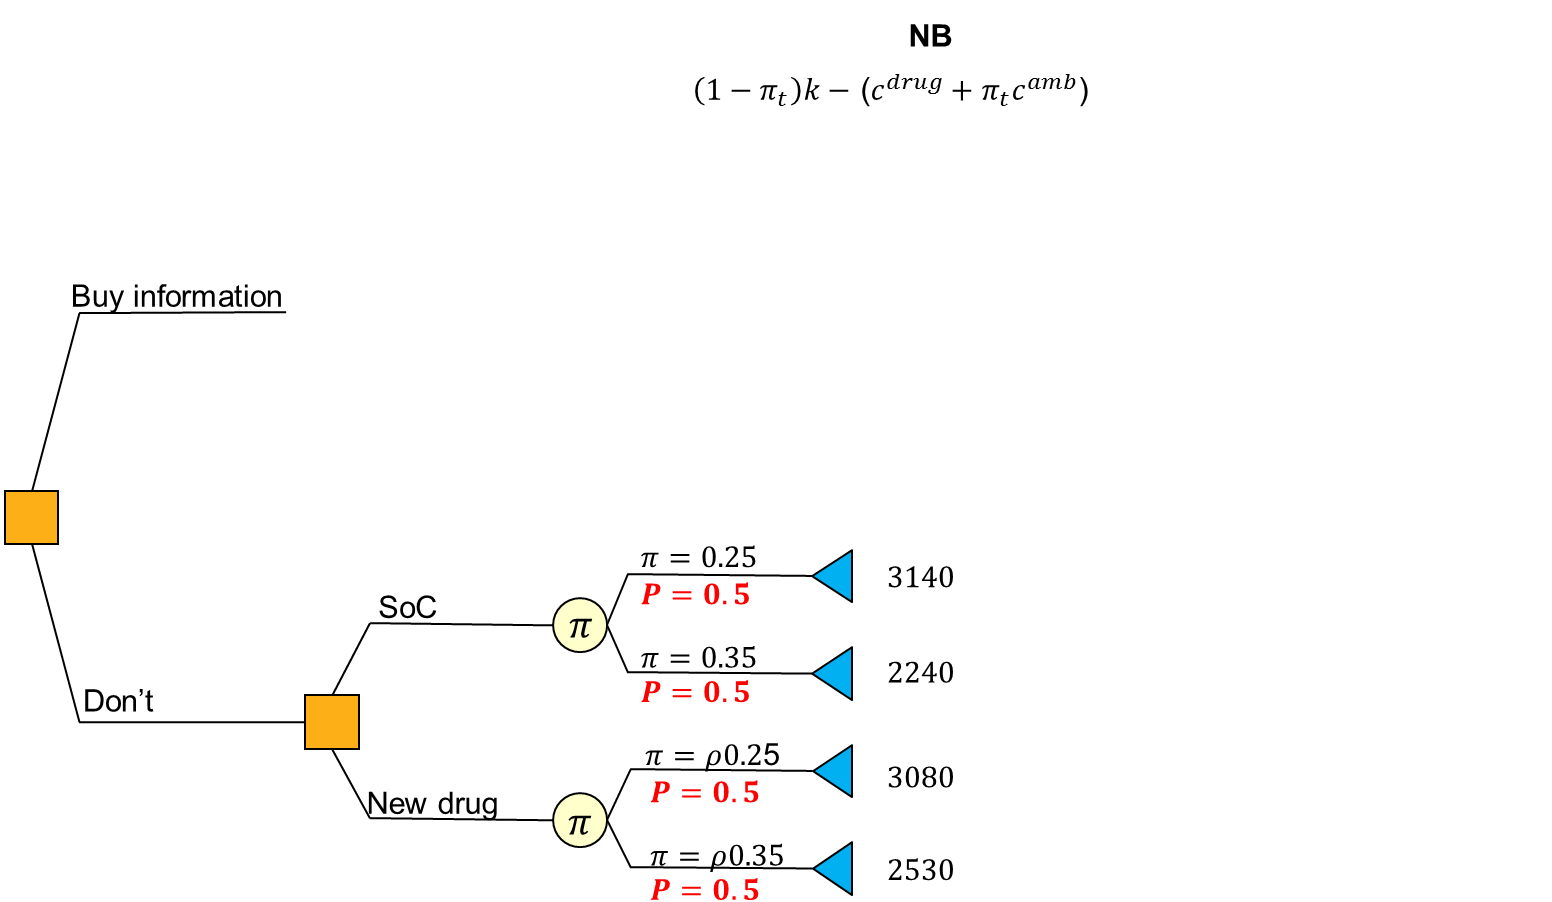
\includegraphics[height=6.5cm]{6.probabilistic-sensitivity-analysis/figs/VPIeg2.png}}}
%%%%%%%%%%%\only<3->{\put(0,0){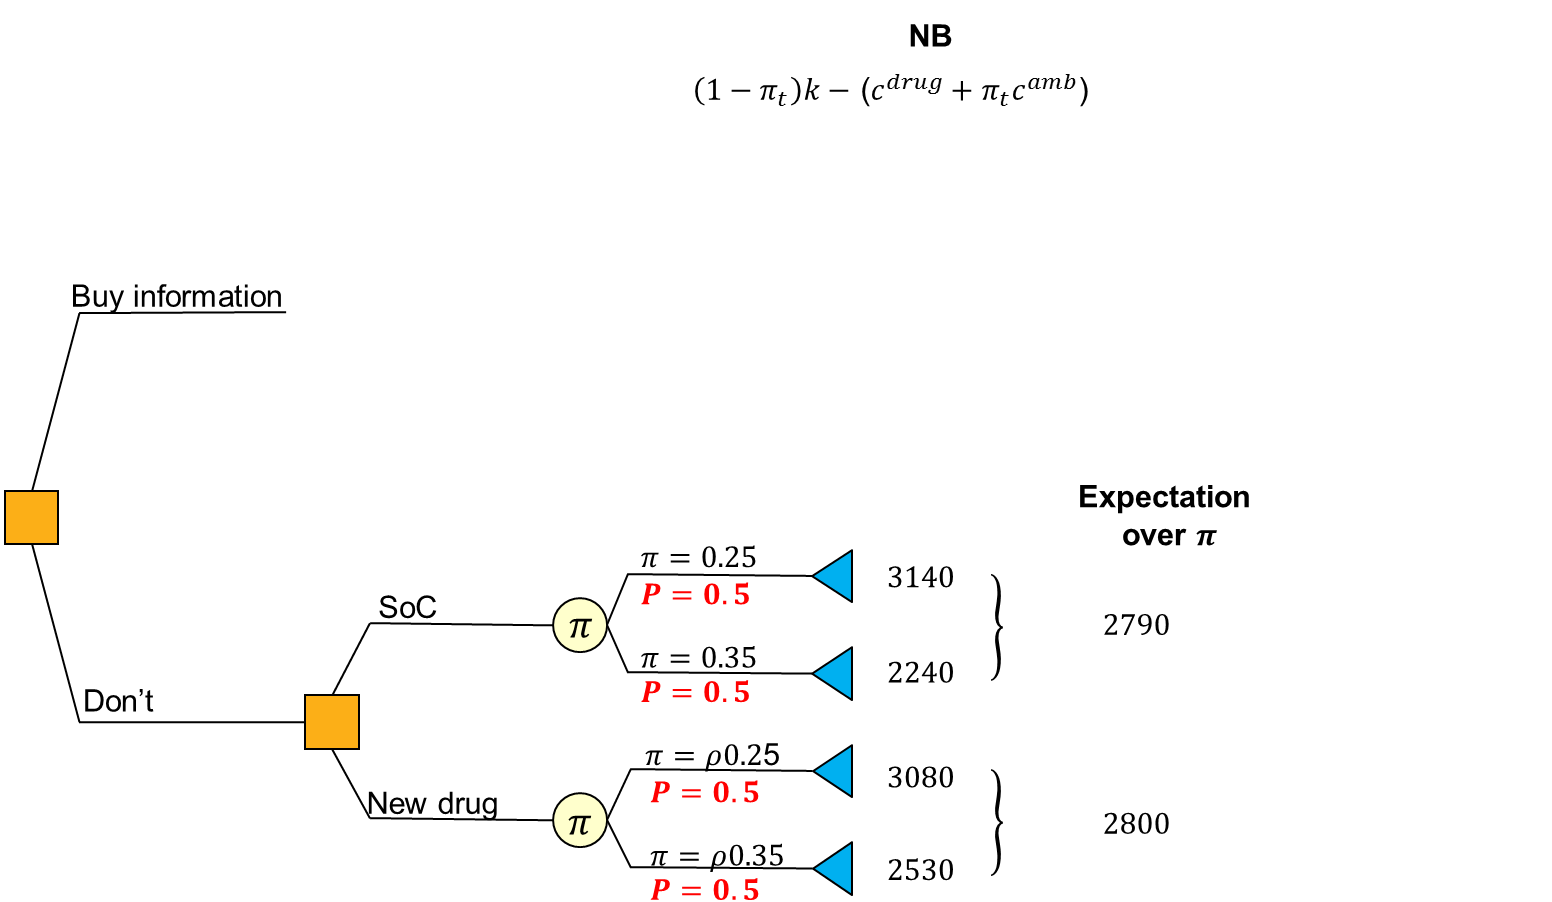
\includegraphics[height=6.5cm]{6.probabilistic-sensitivity-analysis/figs/VPIeg3.png}}}
%%%%%%%%%%%\only<4->{\put(0,0){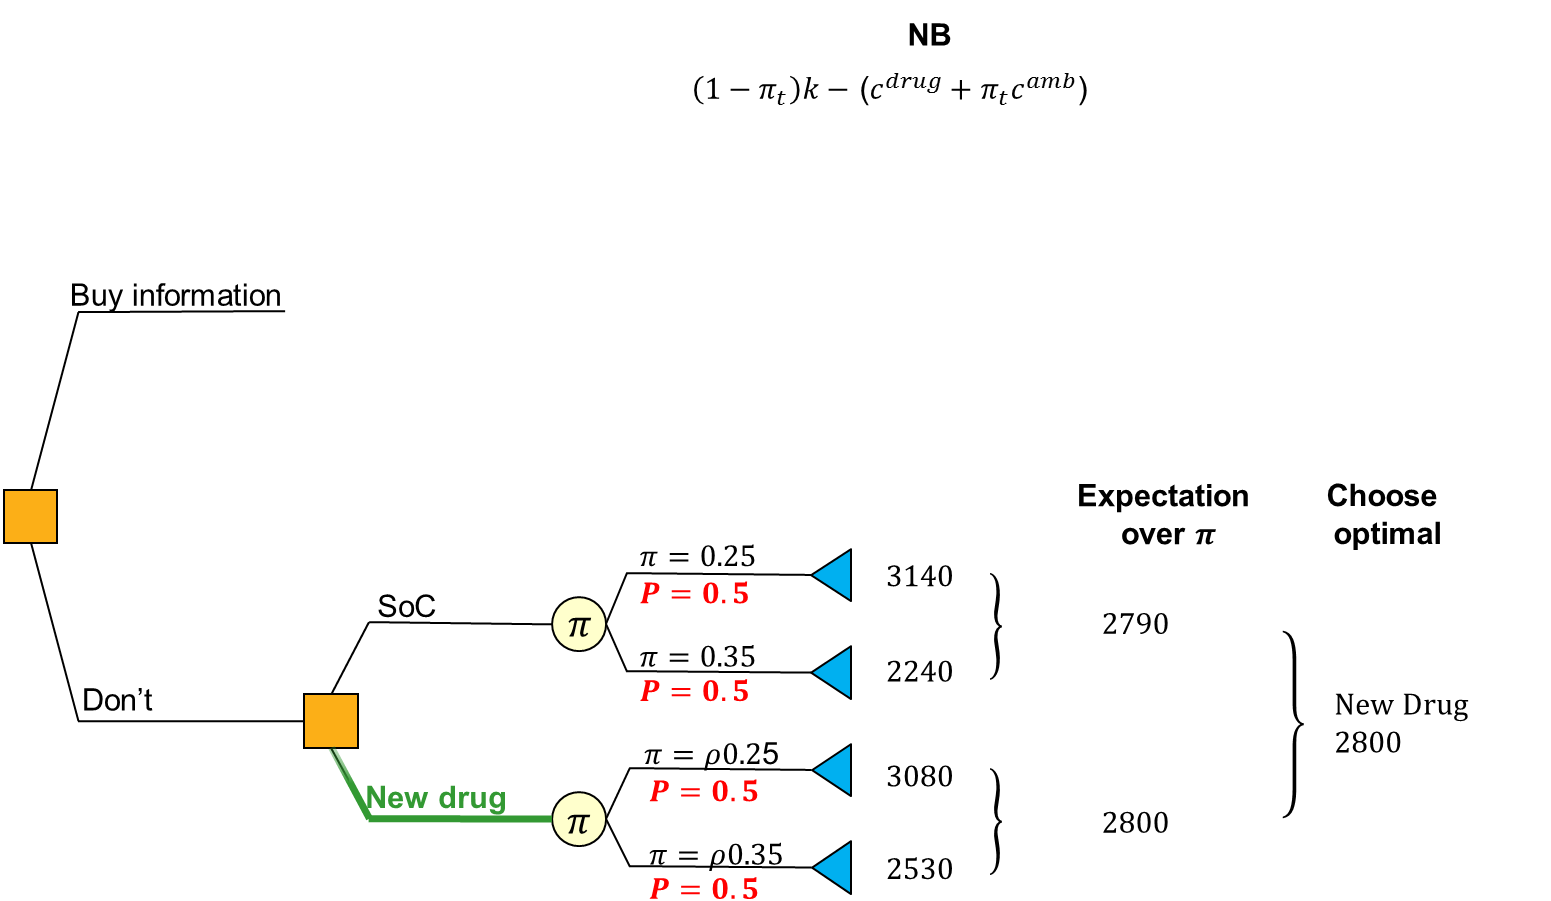
\includegraphics[height=6.5cm]{6.probabilistic-sensitivity-analysis/figs/VPIeg4.png}}}
%%%%%%%%%%%\only<5->{\put(0,0){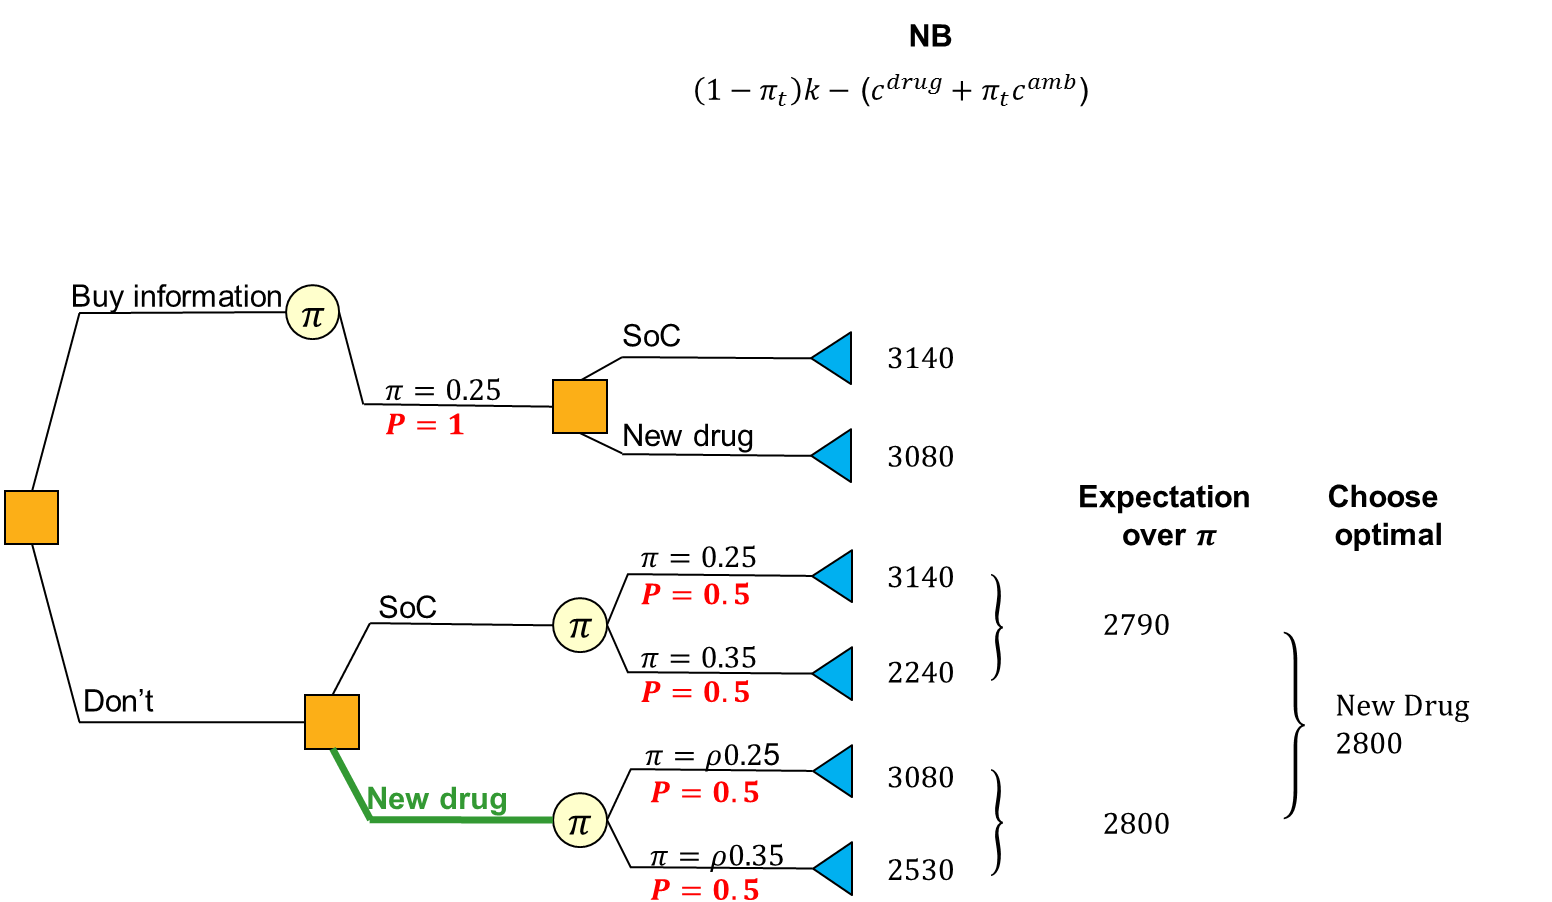
\includegraphics[height=6.5cm]{6.probabilistic-sensitivity-analysis/figs/VPIeg5.png}}}
%%%%%%%%%%%\only<6->{\put(0,0){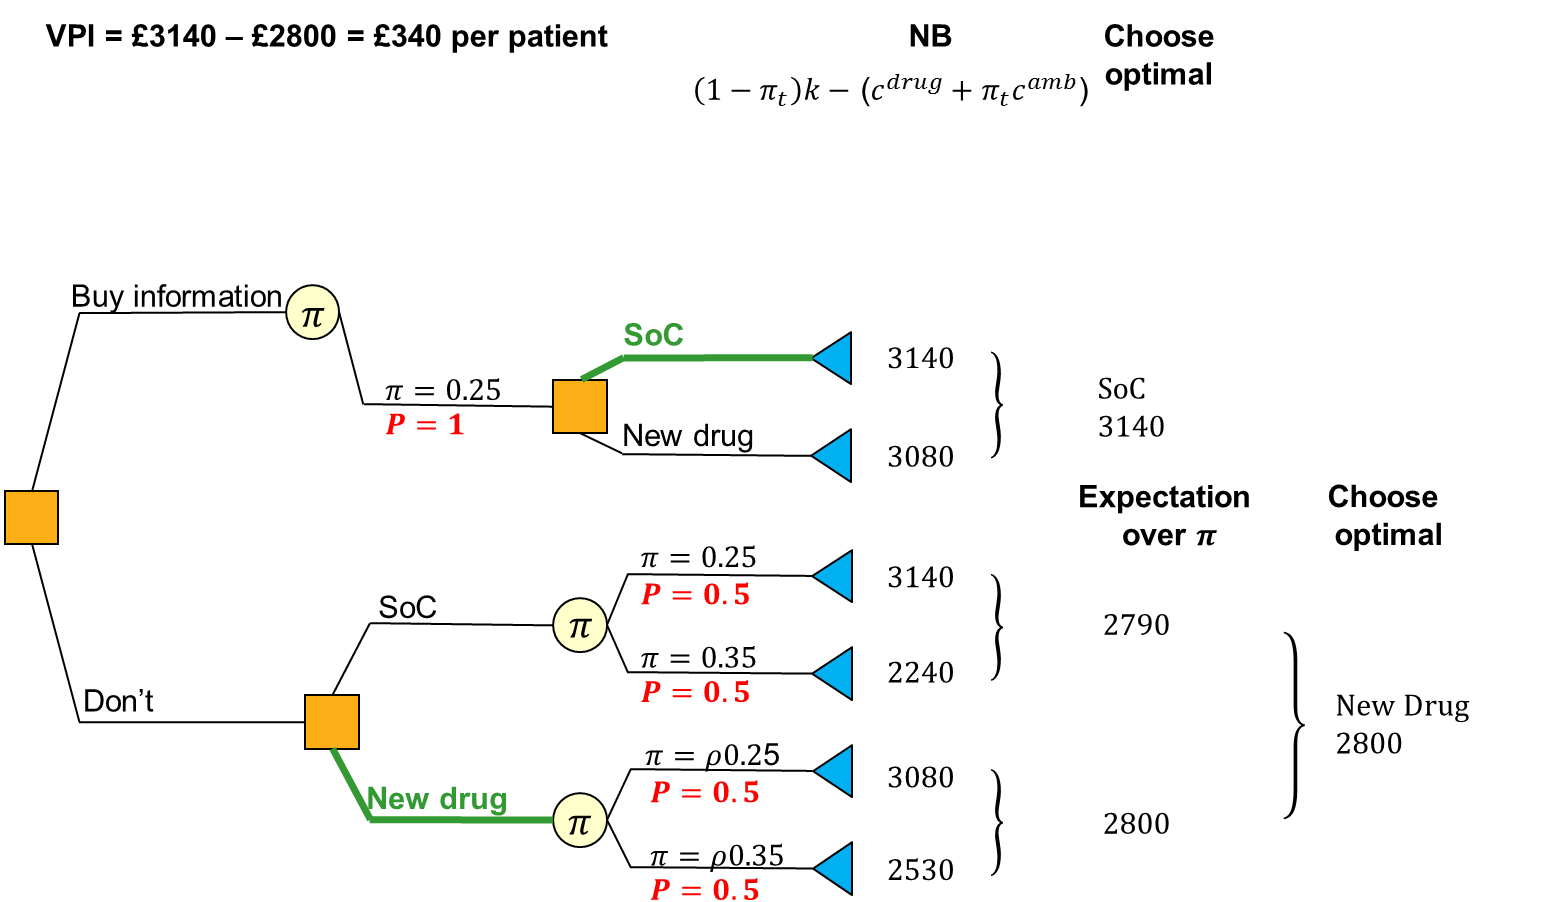
\includegraphics[height=6.5cm]{6.probabilistic-sensitivity-analysis/figs/VPIeg6.png}}}
%%%%%%%%%%%\end{overpic}
%%%%%%%%%%%\end{center}
%%%%%%%%%%%
%%%%%%%%%%%
%%%%%%%%%%%\end{frame}
%%%%%%%%%%%
%%%%%%%%%%%%### New page ############################################################
%%%%%%%%%%%
%%%%%%%%%%%\begin{frame}
%%%%%%%%%%%
%%%%%%%%%%%\frametitle{Expected value of perfect information (EVPI)}
%%%%%%%%%%%{\small
%%%%%%%%%%%\bi
%%%%%%%%%%%\item Perfect information is a hypothetical concept as we don't know the parameter value when deciding to buy it.
%%%%%%%%%%%\item Instead we find the expected NB, averaging over the possible values of $\pi$
%%%%%%%%%%%    \bi
%%%%%%%%%%%    \item $\mathbb{E}_{\pi}[\max_t NB(\pi, t)]$
%%%%%%%%%%%    \ei
%%%%%%%%%%%\item The \alert{expected} value of knowing this infomation is $\mathbb{E}_{\pi}[\max_t NB(\pi; t)] -  \max_t \mathbb{E}_{\pi}(NB(\pi; t)]$
%%%%%%%%%%%\item This is called the Expected Value of Perfect Information (EVPI)
%%%%%%%%%%%\item Note that, if for every value of $\pi$ we don't change the treatment decision, then the EVPI is zero
%%%%%%%%%%%\ei
%%%%%%%%%%%
%%%%%%%%%%%\begin{block}{Golden rule of Value of Information}
%%%%%%%%%%%Information only has value if it changes your decision
%%%%%%%%%%%\end{block}
%%%%%%%%%%%
%%%%%%%%%%%}
%%%%%%%%%%%
%%%%%%%%%%%\end{frame}
%%%%%%%%%%%
%%%%%%%%%%%
%%%%%%%%%%%%### New page ############################################################
%%%%%%%%%%%
%%%%%%%%%%%\begin{frame}
%%%%%%%%%%%
%%%%%%%%%%%\frametitle{Expected value of perfect information (EVPI)}
%%%%%%%%%%%
%%%%%%%%%%%\begin{center}
%%%%%%%%%%%\begin{overpic}[height=6.5cm]{6.probabilistic-sensitivity-analysis/figs/EVPIeg1.png}
%%%%%%%%%%%\only<2->{\put(0,0){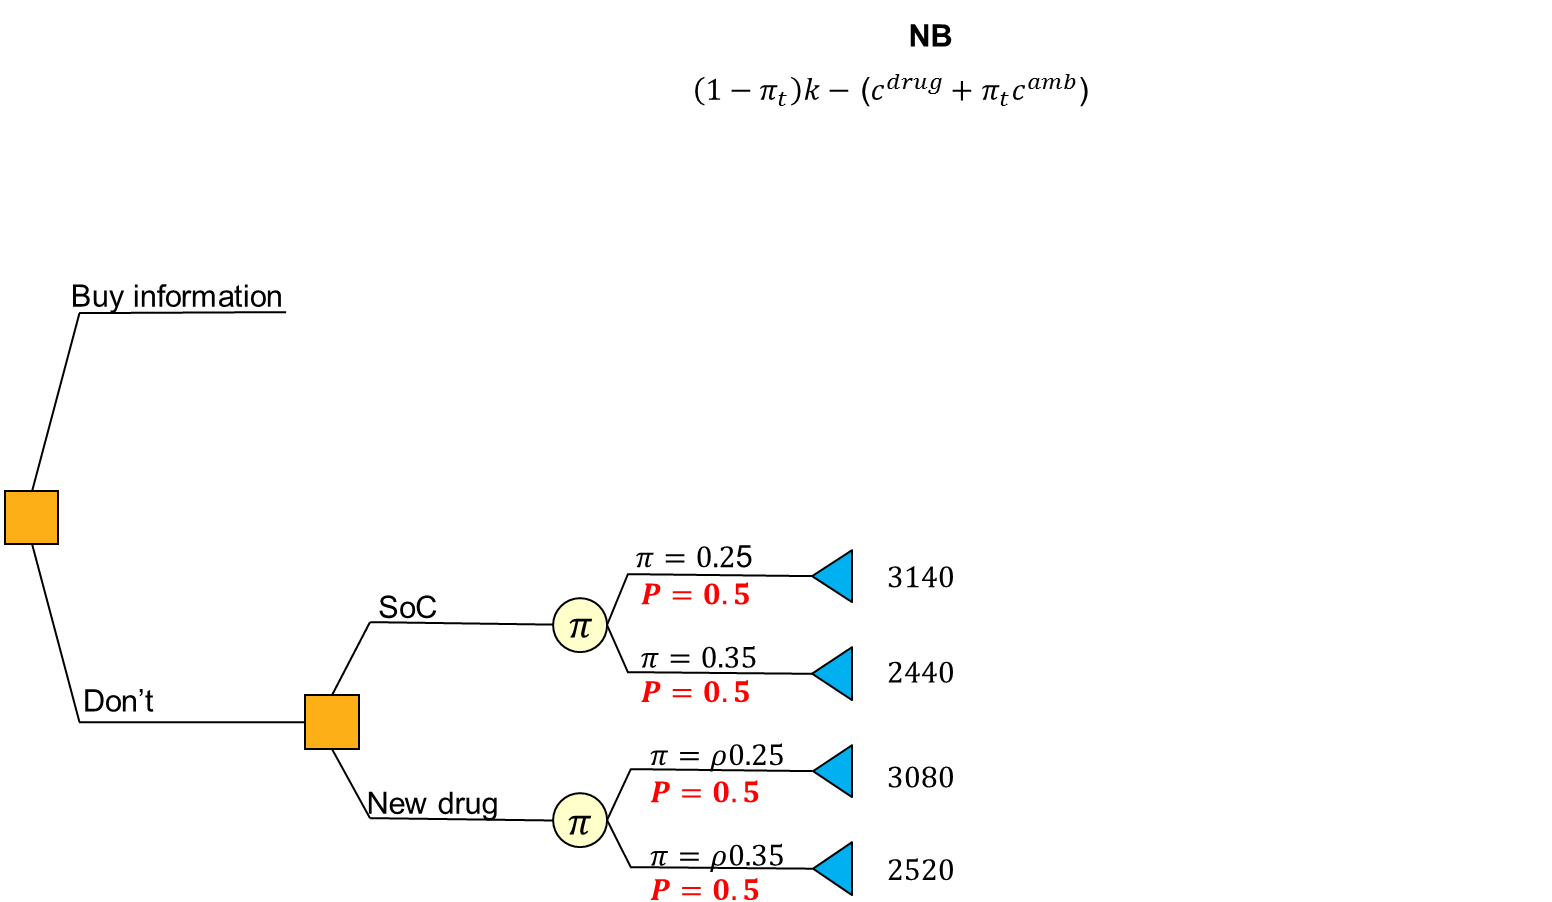
\includegraphics[height=6.5cm]{6.probabilistic-sensitivity-analysis/figs/EVPIeg2.png}}}
%%%%%%%%%%%\only<3->{\put(0,0){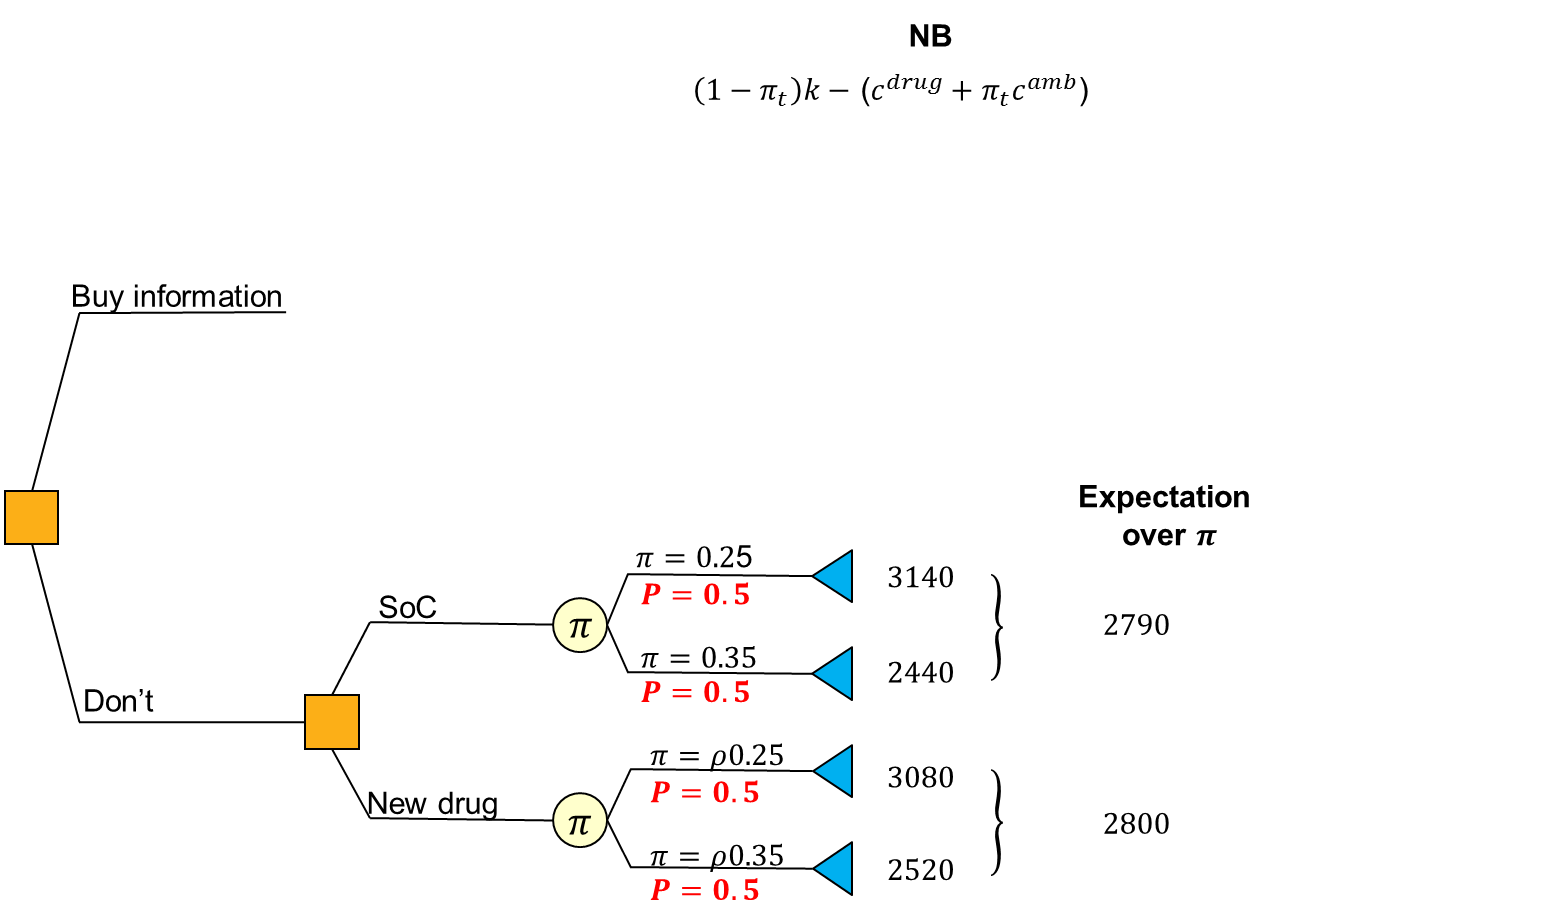
\includegraphics[height=6.5cm]{6.probabilistic-sensitivity-analysis/figs/EVPIeg3.png}}}
%%%%%%%%%%%\only<4->{\put(0,0){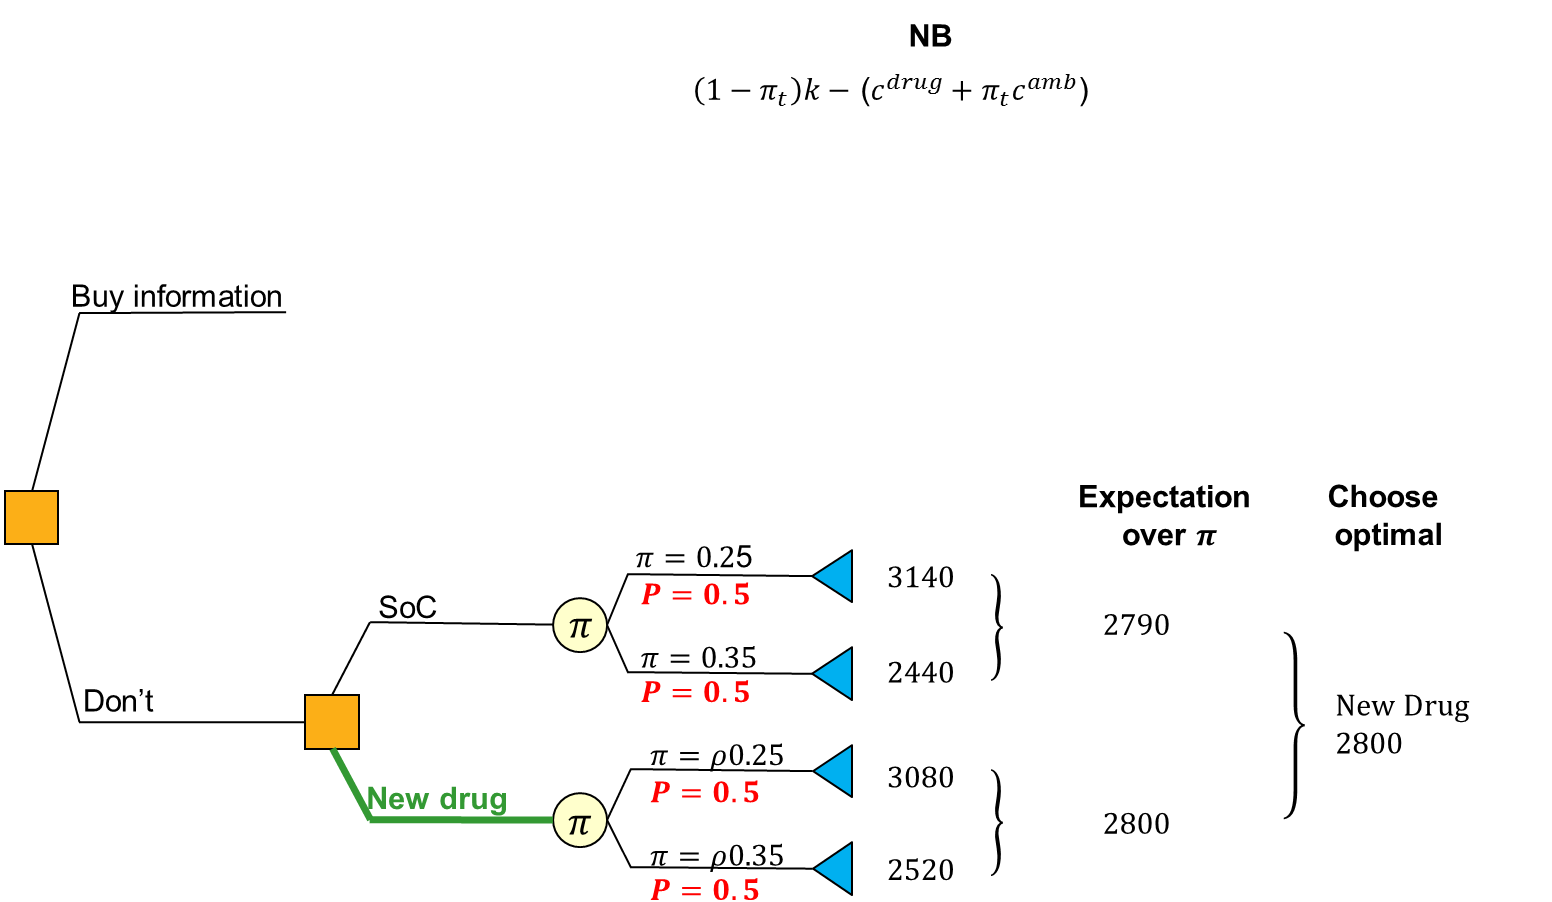
\includegraphics[height=6.5cm]{6.probabilistic-sensitivity-analysis/figs/EVPIeg4.png}}}
%%%%%%%%%%%\only<5->{\put(0,0){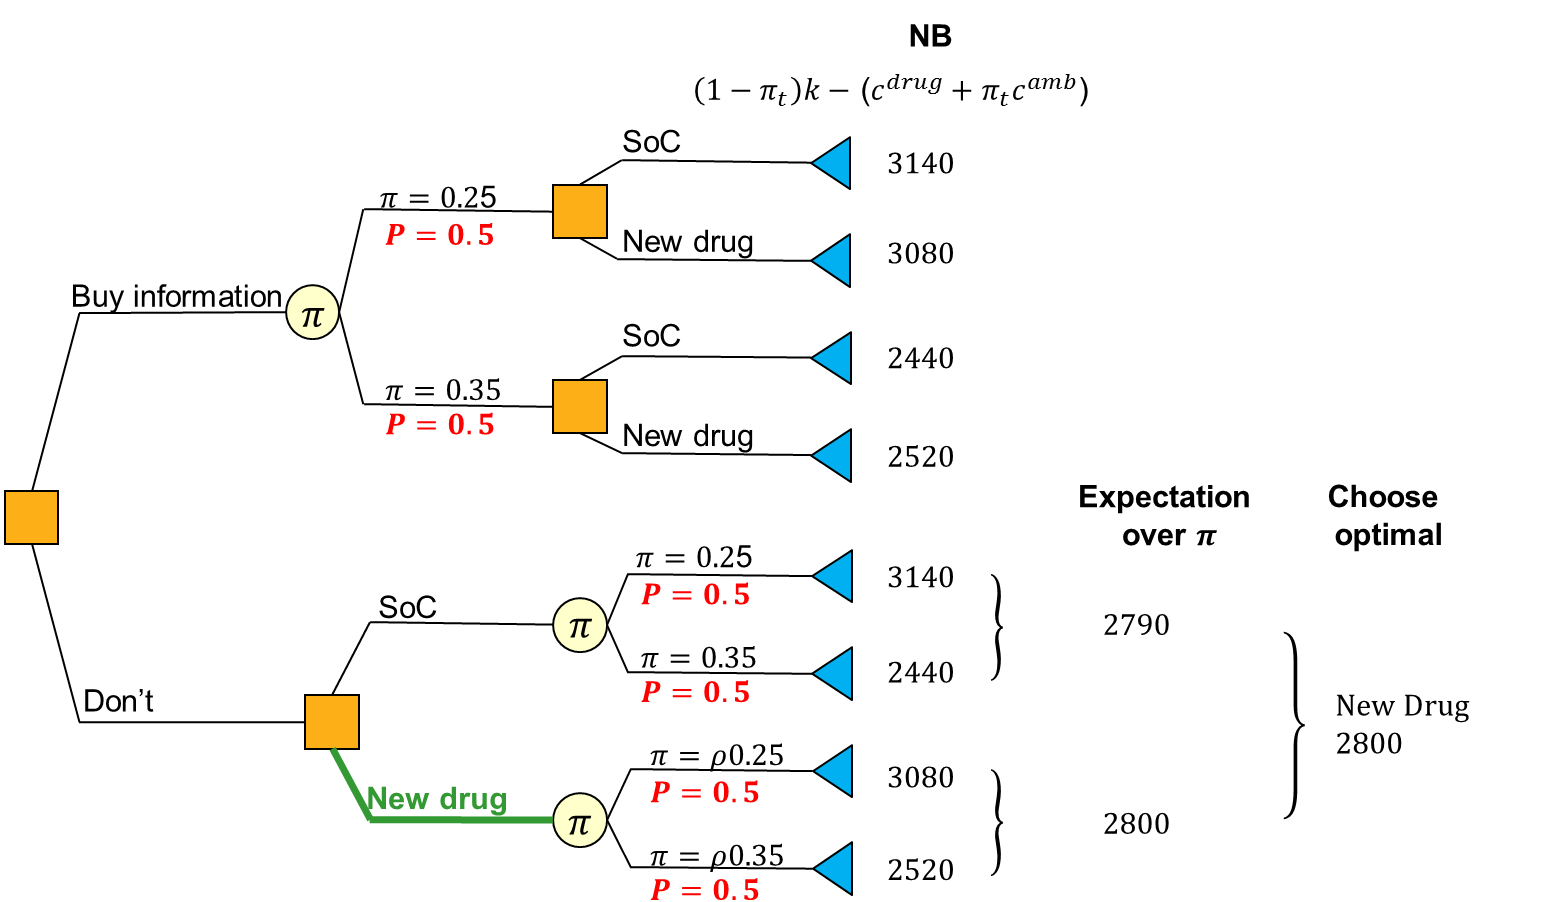
\includegraphics[height=6.5cm]{6.probabilistic-sensitivity-analysis/figs/EVPIeg5.png}}}
%%%%%%%%%%%\only<6->{\put(0,0){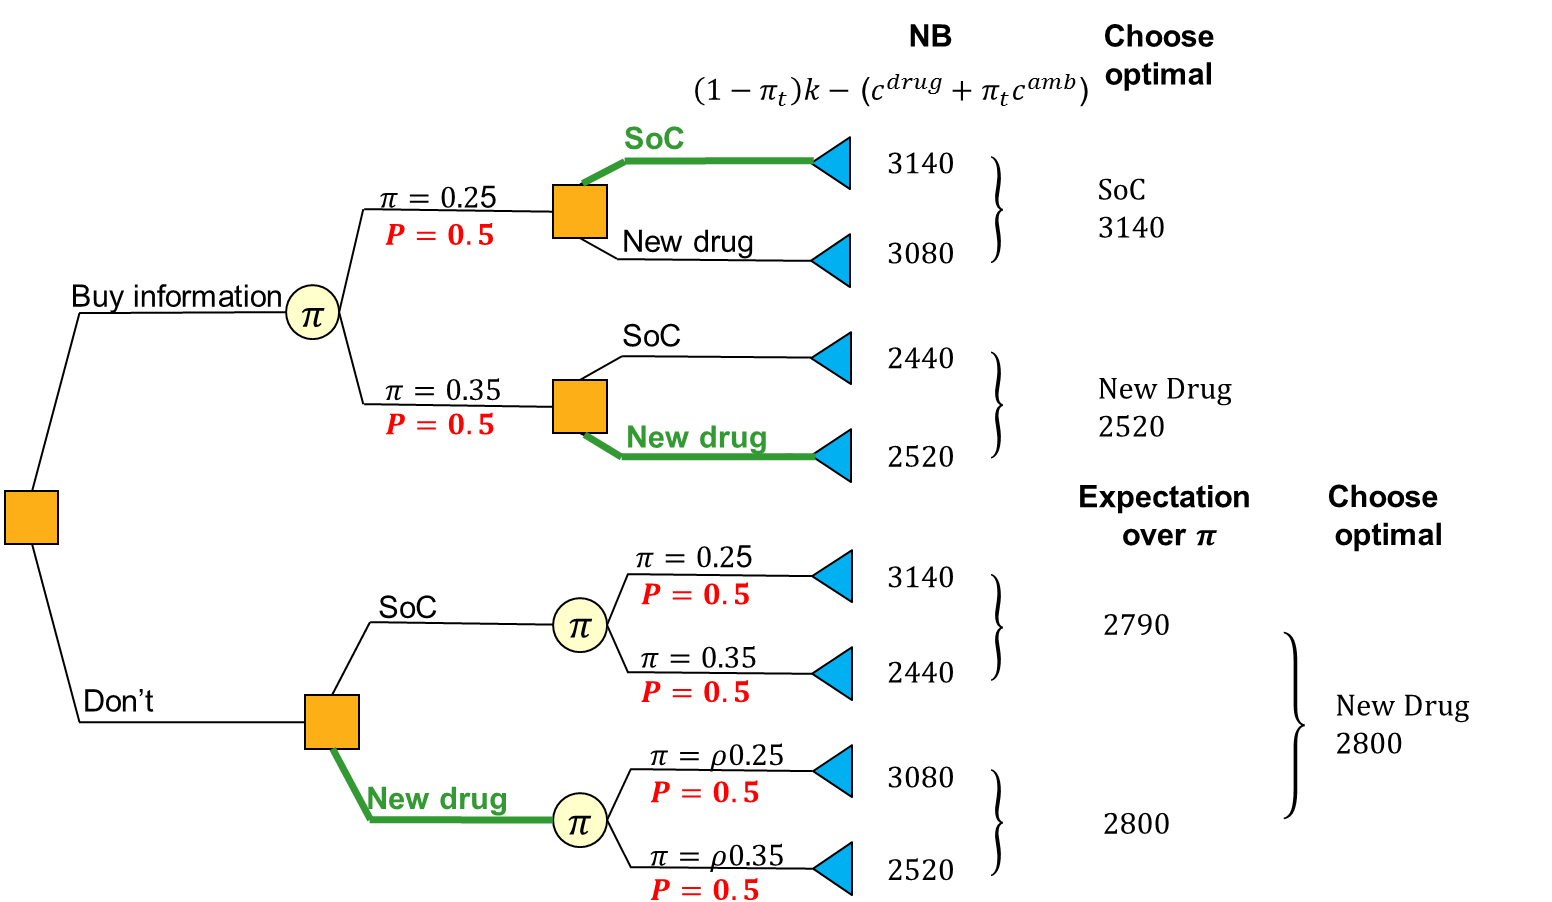
\includegraphics[height=6.5cm]{6.probabilistic-sensitivity-analysis/figs/EVPIeg6.png}}}
%%%%%%%%%%%\only<7->{\put(0,0){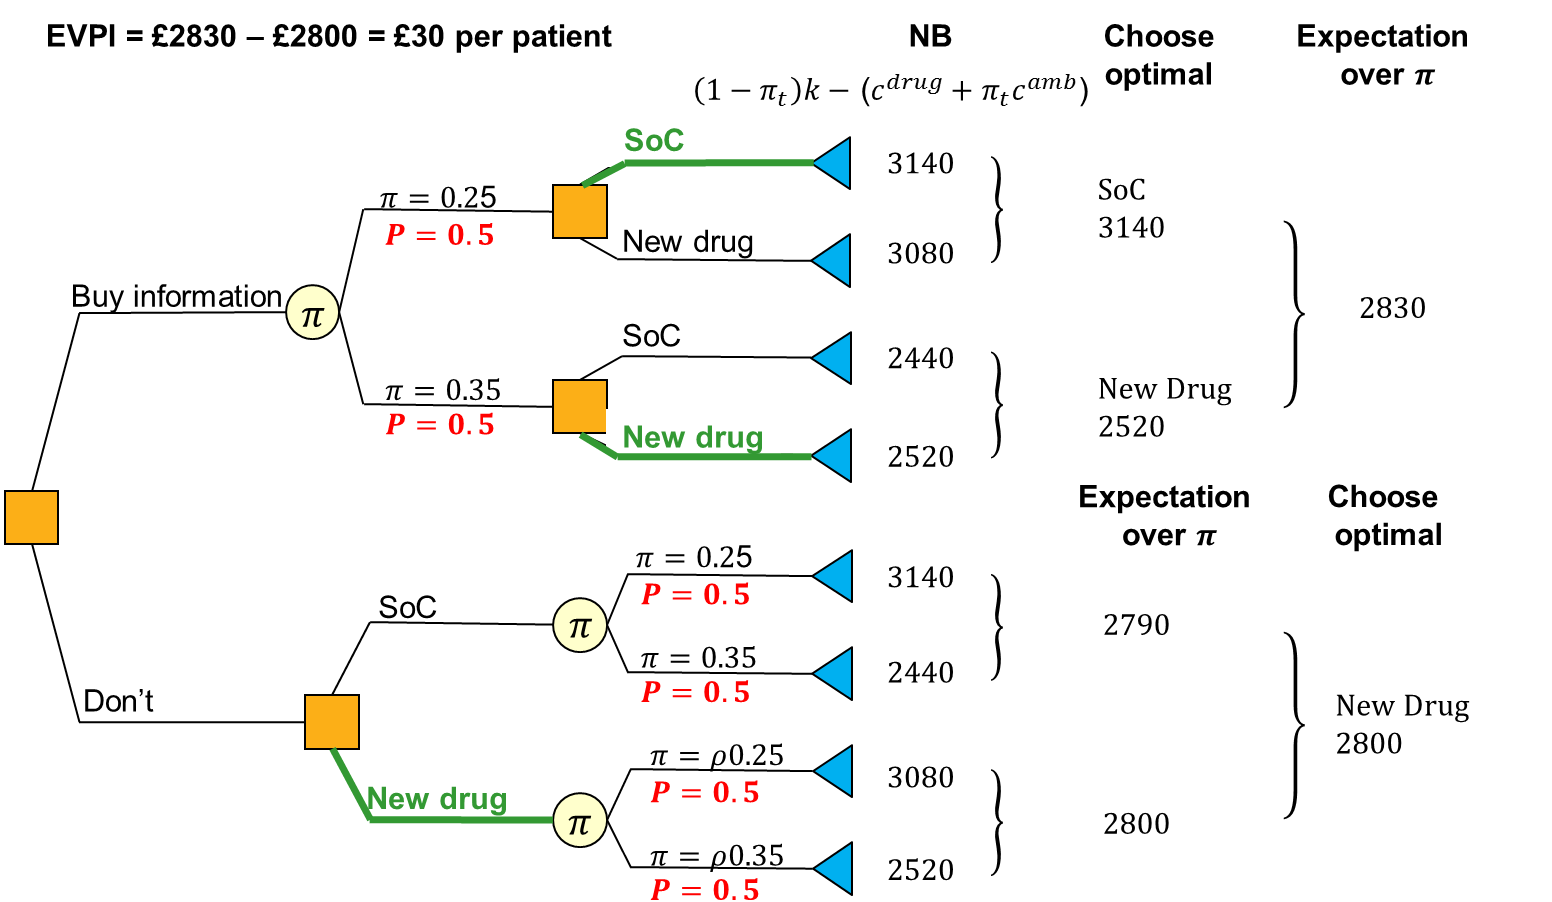
\includegraphics[height=6.5cm]{6.probabilistic-sensitivity-analysis/figs/EVPIeg7.png}}}
%%%%%%%%%%%\end{overpic}
%%%%%%%%%%%\end{center}
%%%%%%%%%%%
%%%%%%%%%%%
%%%%%%%%%%%\end{frame}
%%%%%%%%%%%
%%%%%%%%%%%
%%%%%%%%%%%%### New page ############################################################
%%%%%%%%%%%
%%%%%%%%%%%\begin{frame}
%%%%%%%%%%%
%%%%%%%%%%%\frametitle{Expected value of perfect information (EVPI)}
%%%%%%%%%%%
%%%%%%%%%%%\begin{center}
%%%%%%%%%%%\begin{overpic}[height=6.5cm]{6.probabilistic-sensitivity-analysis/figs/EVPI1.png}
%%%%%%%%%%%\only<2->{\put(0,0){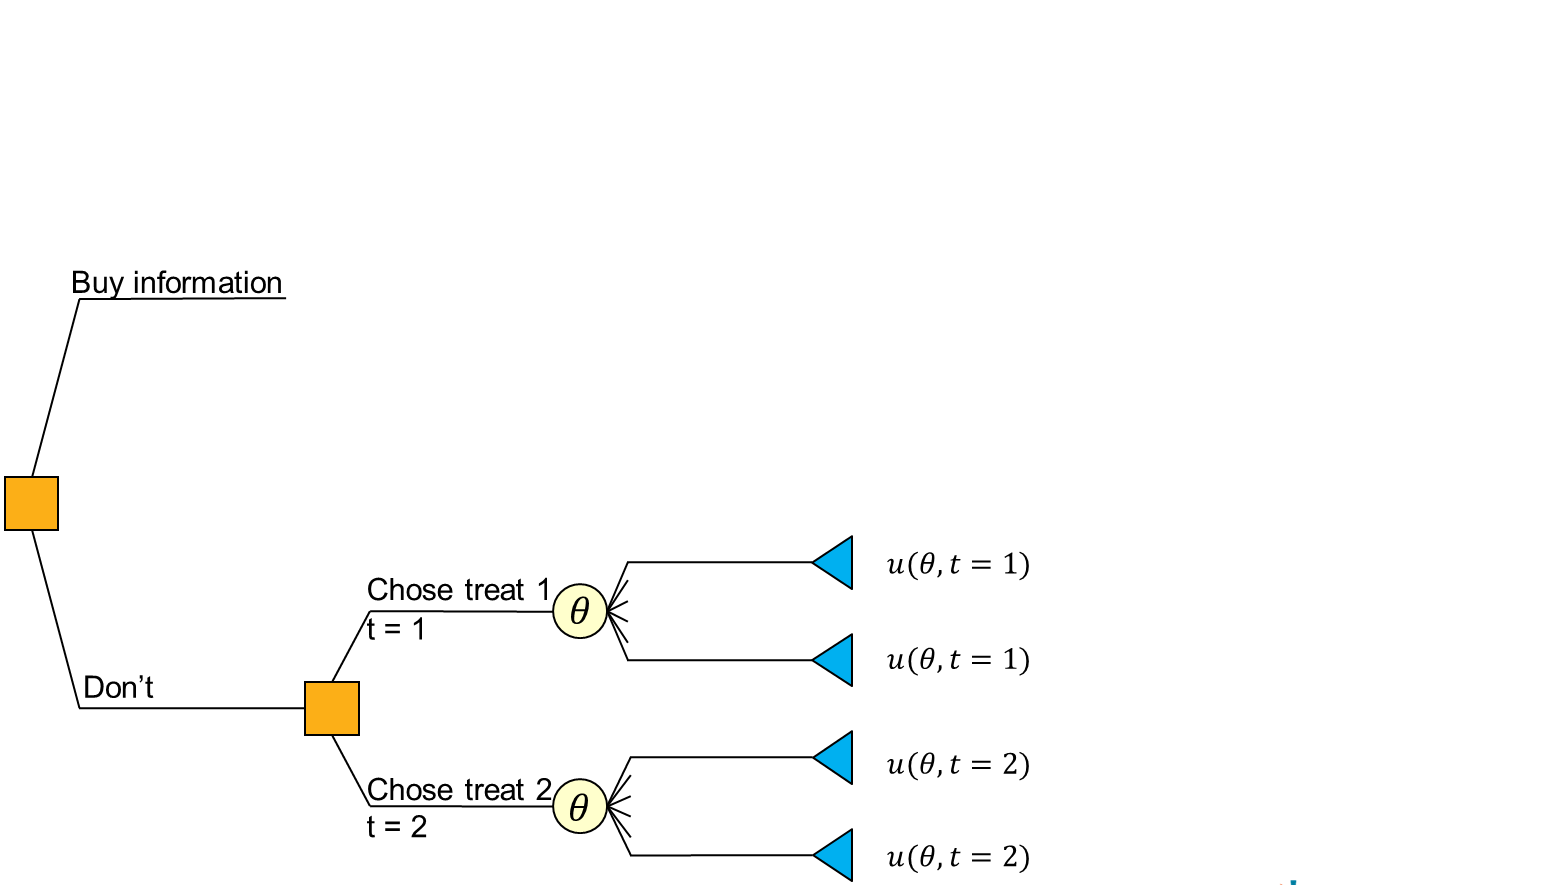
\includegraphics[height=6.5cm]{6.probabilistic-sensitivity-analysis/figs/EVPI2.png}}}
%%%%%%%%%%%\only<3->{\put(0,0){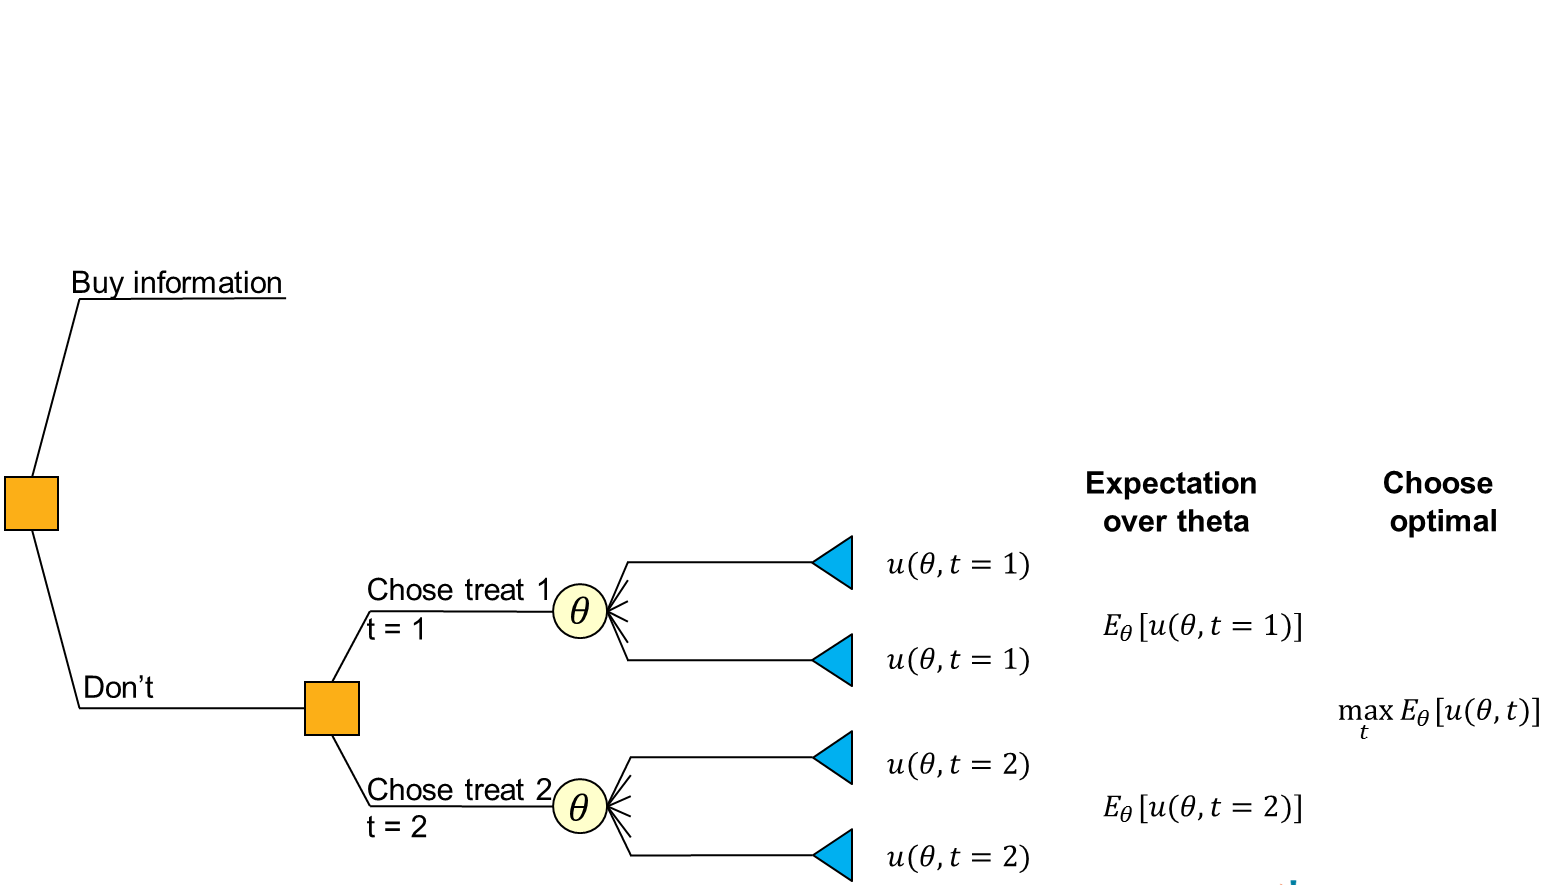
\includegraphics[height=6.5cm]{6.probabilistic-sensitivity-analysis/figs/EVPI3.png}}}
%%%%%%%%%%%\only<4->{\put(0,0){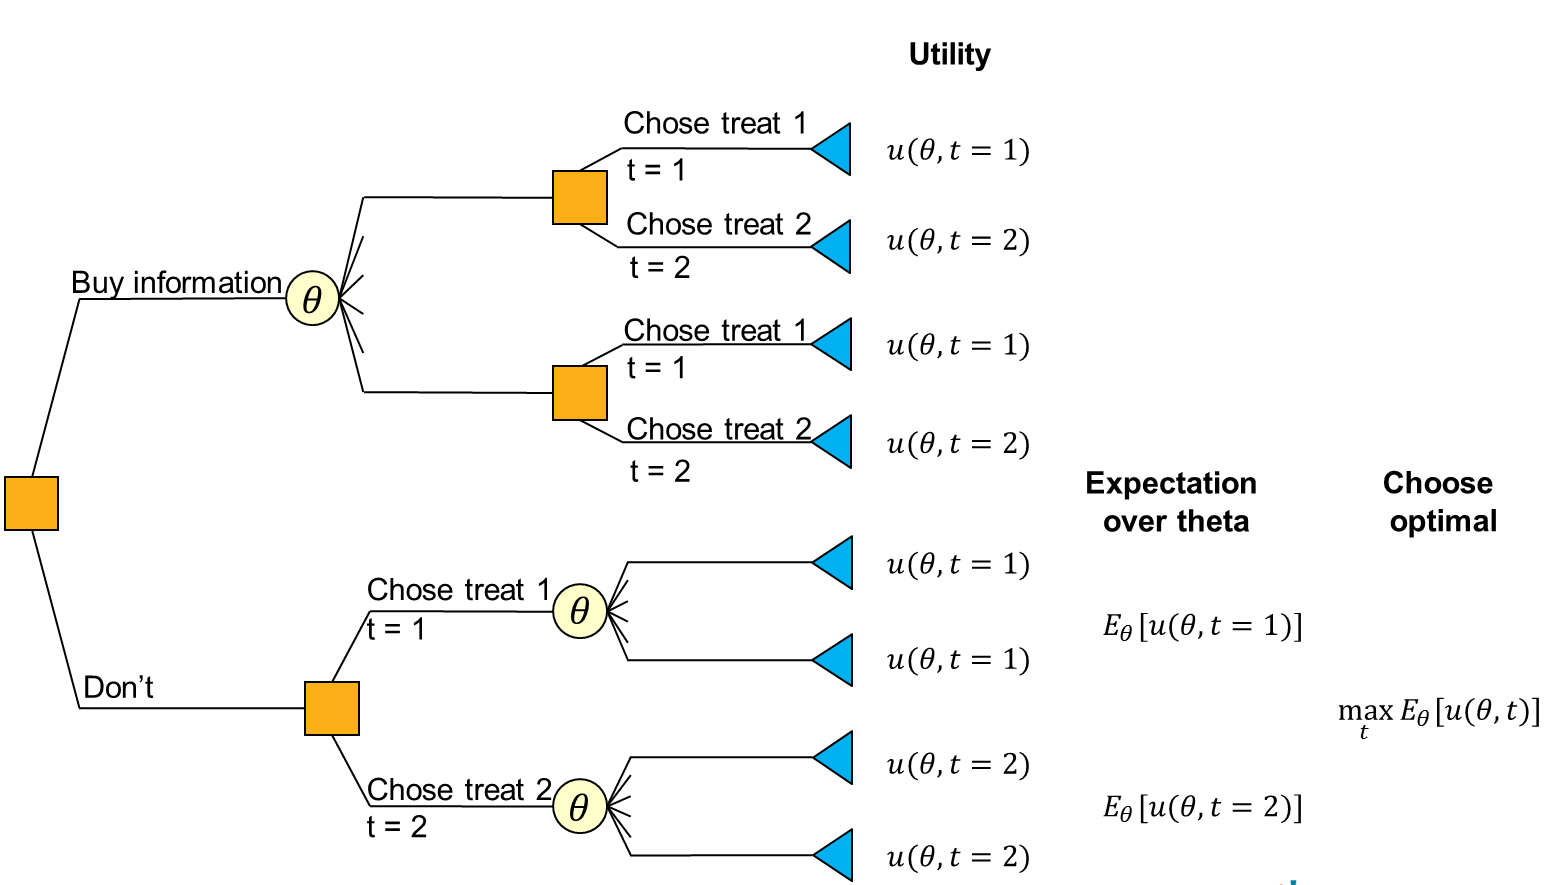
\includegraphics[height=6.5cm]{6.probabilistic-sensitivity-analysis/figs/EVPI4.png}}}
%%%%%%%%%%%\only<5->{\put(0,0){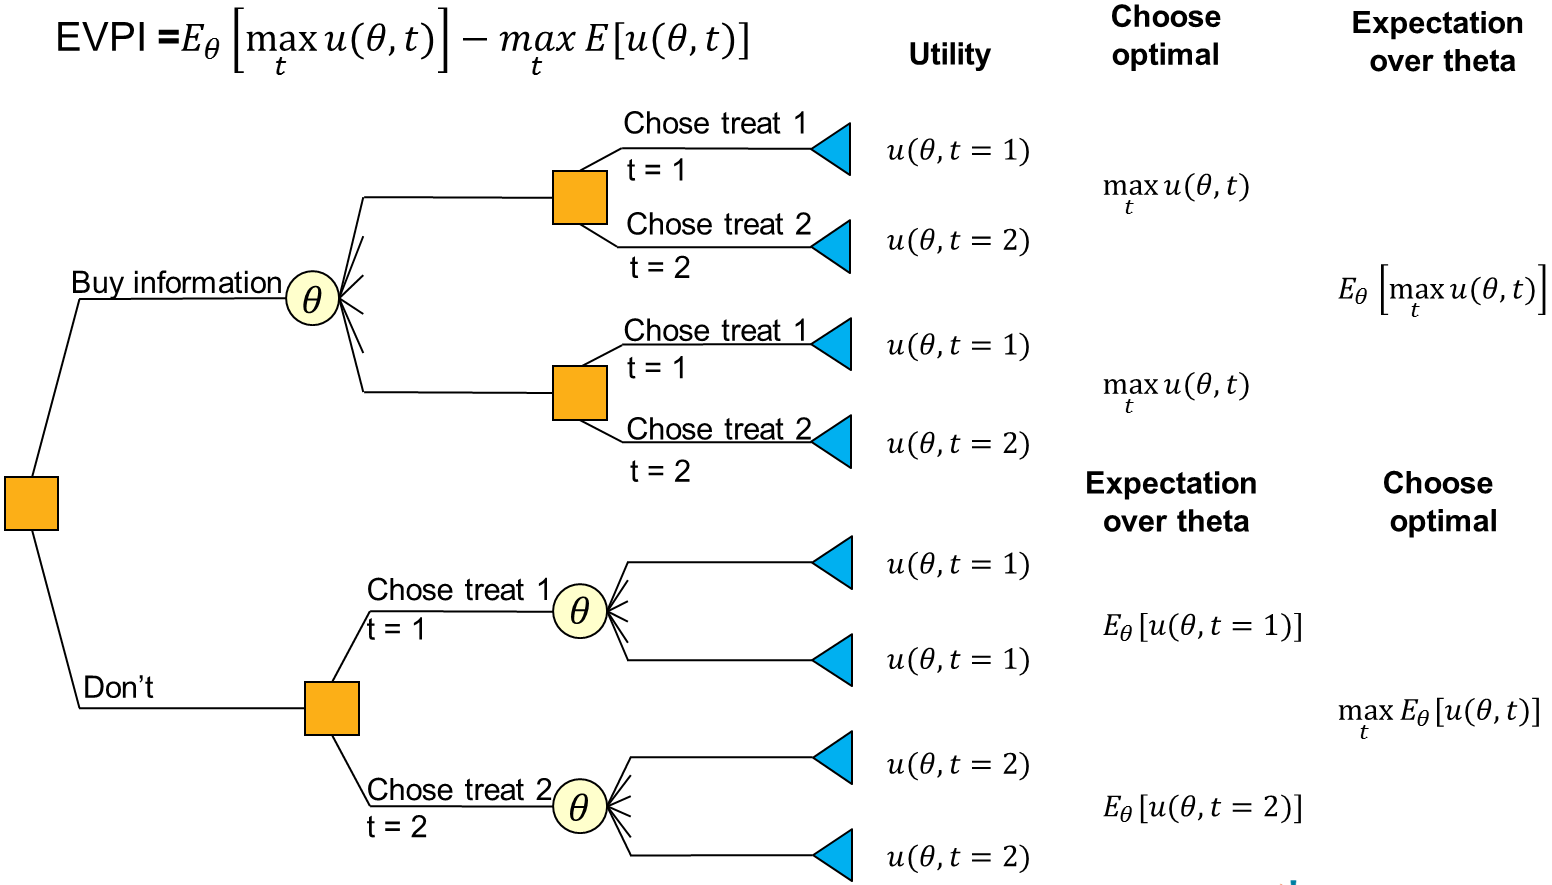
\includegraphics[height=6.5cm]{6.probabilistic-sensitivity-analysis/figs/EVPI5.png}}}
%%%%%%%%%%%\end{overpic}
%%%%%%%%%%%\end{center}
%%%%%%%%%%%
%%%%%%%%%%%
%%%%%%%%%%%\end{frame}
%%%%%%%%%%%
%%%%%%%%%%%%### New page ############################################################
%%%%%%%%%%%
%%%%%%%%%%%\begin{frame}[fragile]
%%%%%%%%%%%
%%%%%%%%%%%\frametitle{How to estimate EVPI by simulation}
%%%%%%%%%%%
%%%%%%%%%%%{\small
%%%%%%%%%%%%\begin{columns}
%%%%%%%%%%%%\column{0.47\paperwidth}
%%%%%%%%%%%Decide to \alert{not} buy information\\
%%%%%%%%%%%1) Simulate a set of parameters $\mathbf{\theta} = \theta_1 ,\ldots, \theta_I$\\
%%%%%%%%%%%
%%%%%%%%%%%2) For each treatment $t_k = t_1, \ldots , t_K$\\
%%%%%%%%%%%\hspace{1em} a) Find utility of treatment $t_k$ for each $\theta_i$. $u(\theta_i, t_k)$\\
%%%%%%%%%%%\hspace{1em} b) Estimate $\mathbb{E}_{\theta}\left[u(\theta, t_k)  \right]$ by the mean over $i$ of  $u(\theta_i, t_k)$\\
%%%%%%%%%%%
%%%%%%%%%%%3) The value of the decision is $\max_t\mathbb{E}_{\theta}\left[u(\theta, t)  \right]$\\
%%%%%%%%%%%
%%%%%%%%%%%
%%%%%%%%%%%\vspace{1em}
%%%%%%%%%%%Decision to buy information\\
%%%%%%%%%%%1) Simulate a set of parameters $\mathbf{\theta} = \theta_1 ,\ldots, \theta_I$\\
%%%%%%%%%%%
%%%%%%%%%%%2) For each parameter $\theta_i$\\
%%%%%%%%%%%\hspace{1em} a) Find utility of  $\theta_i$ for each treatment $t_k = t_1, \ldots , t_K$. $u(\theta_i, t_k)$\\
%%%%%%%%%%%\hspace{1em} b) Choose treatment $t^*$ that is $\max_t u(\theta_i, t_k)$\\
%%%%%%%%%%%
%%%%%%%%%%%3) Value of decision is $\mathbb{E}_{\theta}\left[\max_t u(\theta, t)  \right]$ which is estimated by the mean over $i$ of $\max_t u(\theta_i, t^*)$\\
%%%%%%%%%%%
%%%%%%%%%%%\vspace{1em}
%%%%%%%%%%%\[
%%%%%%%%%%%\mbox{EVPI} = \mathbb{E}_{\theta}\left[\max_t u(\theta; t)  \right] - \max_t\mathbb{E}_{\theta}\left[u(\theta; t)  \right]
%%%%%%%%%%%\]
%%%%%%%%%%%
%%%%%%%%%%%%\column{0.47\paperwidth}
%%%%%%%%%%%%\end{columns}
%%%%%%%%%%%}
%%%%%%%%%%%
%%%%%%%%%%%\end{frame}
%%%%%%%%%%%
%%%%%%%%%%%%### New page ############################################################
%%%%%%%%%%%
%%%%%%%%%%%\begin{frame}
%%%%%%%%%%%
%%%%%%%%%%%\frametitle{Expected value of perfect partial information (EVPPI)}
%%%%%%%%%%%
%%%%%%%%%%%\bi
%%%%%%%%%%%\item Generally we don't want to know the value of knowing all the parameters exactly, but the value of knowing \alert{each} parameter (or a group of parameters), exactly.
%%%%%%%%%%%\item Partition the parameters into two groups
%%%%%%%%%%%    \bi
%%%%%%%%%%%    \item $\theta = (\phi, \psi)$
%%%%%%%%%%%    \ei
%%%%%%%%%%%\item We want to know the value of knowing $\phi$ perfectly, whilst remaining uncertain about $\psi$
%%%%%%%%%%%\ei
%%%%%%%%%%%
%%%%%%%%%%%\end{frame}
%%%%%%%%%%%
%%%%%%%%%%%%### New page ############################################################
%%%%%%%%%%%
%%%%%%%%%%%\begin{frame}
%%%%%%%%%%%
%%%%%%%%%%%\frametitle{Expected value of perfect partial information (EVPPI)}
%%%%%%%%%%%
%%%%%%%%%%%\begin{center}
%%%%%%%%%%%\begin{overpic}[height=6.5cm]{6.probabilistic-sensitivity-analysis/figs/EVPPI1.png}
%%%%%%%%%%%\only<2->{\put(0,0){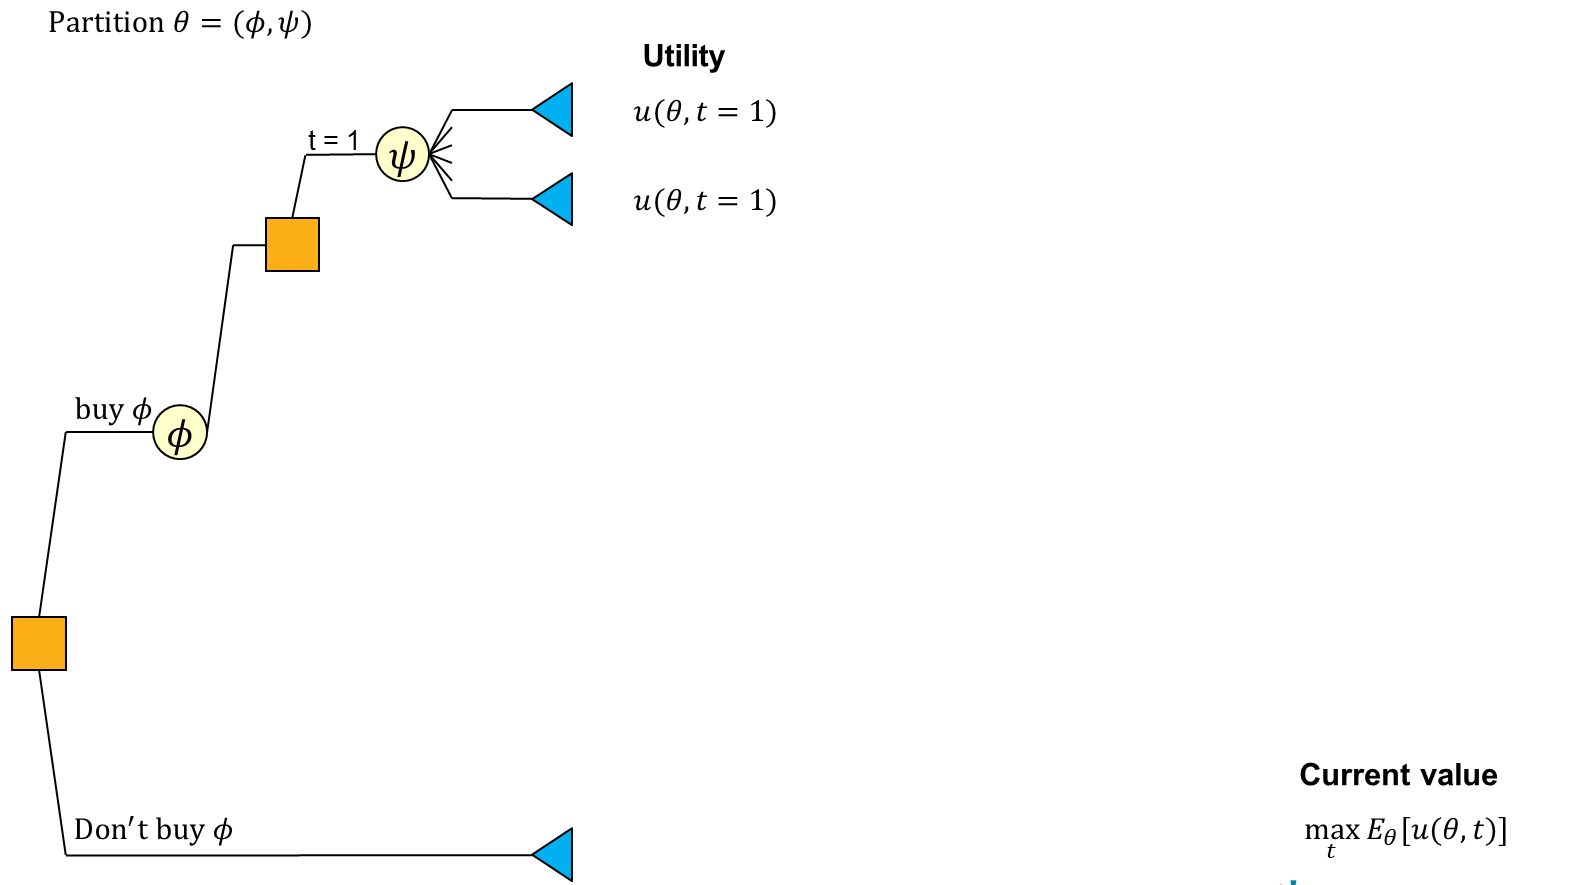
\includegraphics[height=6.5cm]{6.probabilistic-sensitivity-analysis/figs/EVPPI2.png}}}
%%%%%%%%%%%\only<3->{\put(0,0){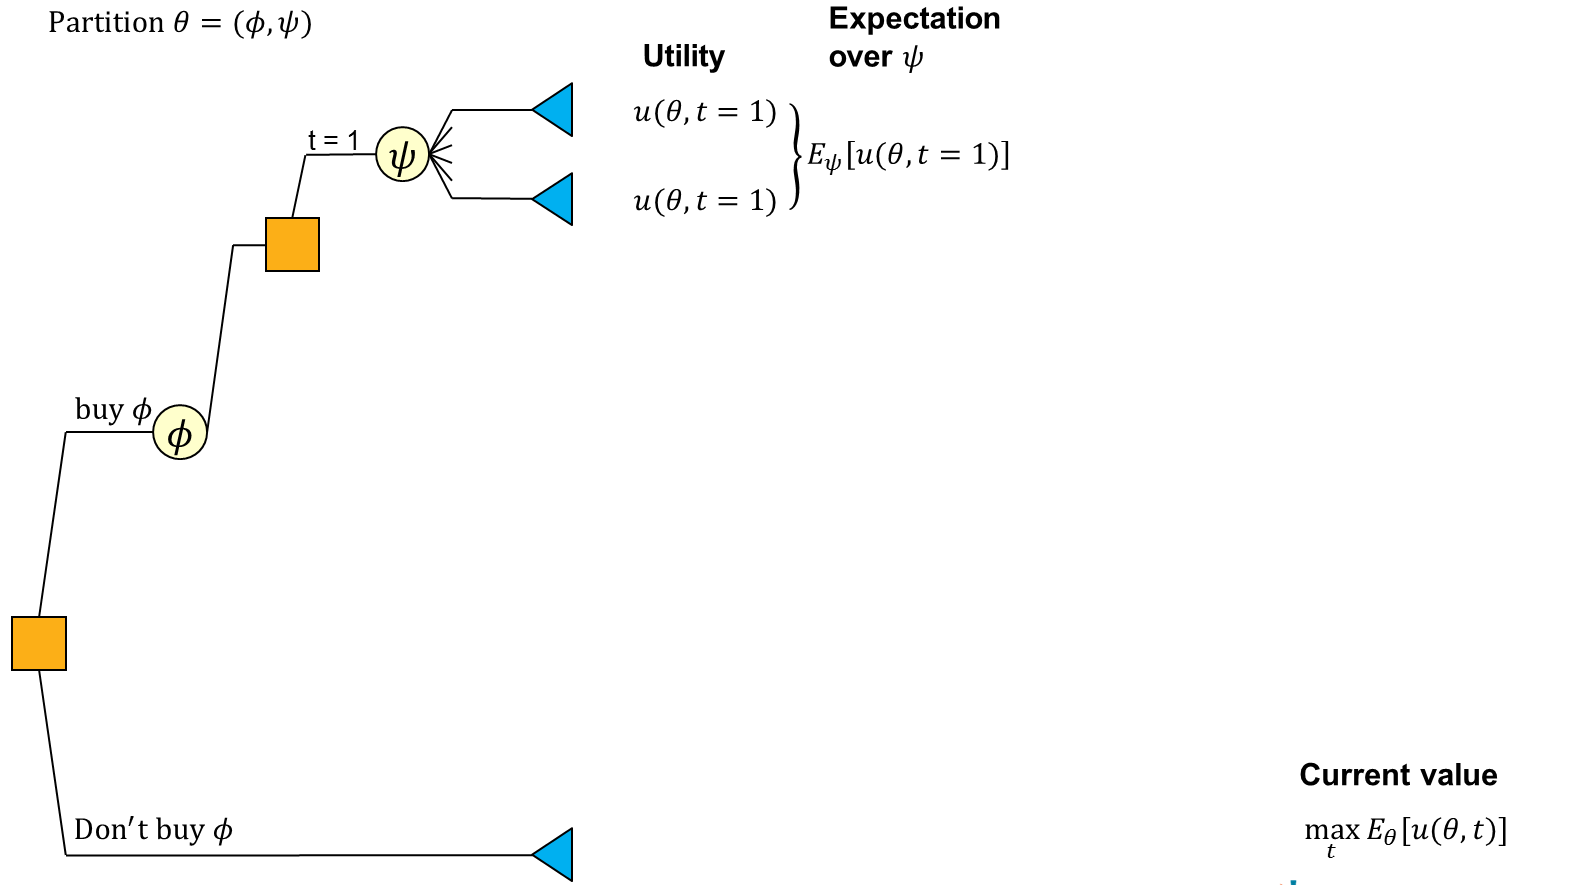
\includegraphics[height=6.5cm]{6.probabilistic-sensitivity-analysis/figs/EVPPI3.png}}}
%%%%%%%%%%%\only<4->{\put(0,0){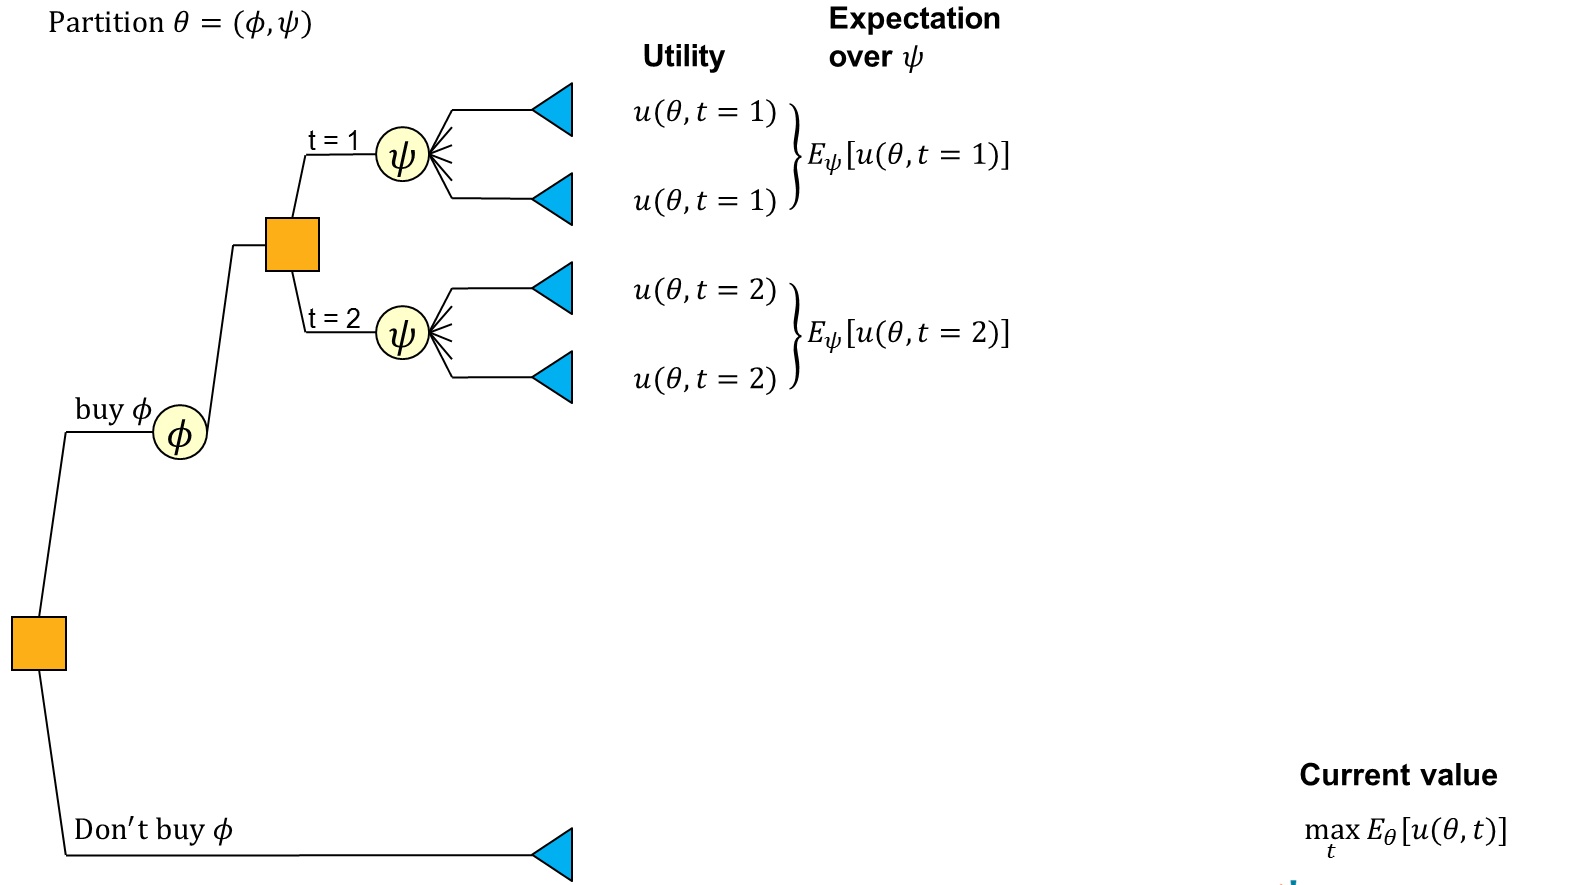
\includegraphics[height=6.5cm]{6.probabilistic-sensitivity-analysis/figs/EVPPI4.png}}}
%%%%%%%%%%%\only<5->{\put(0,0){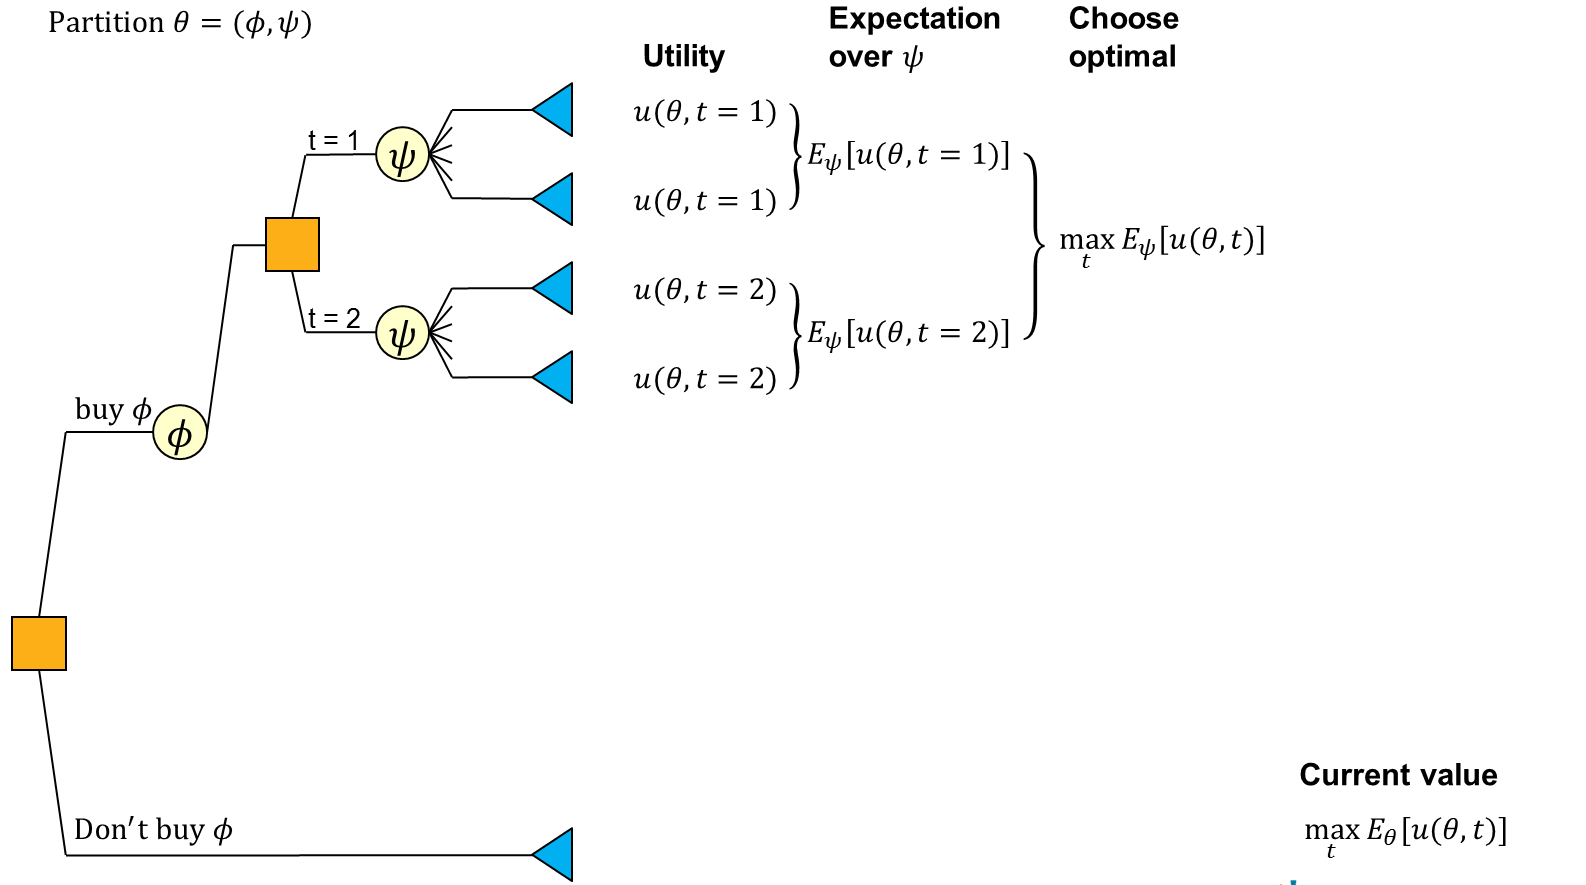
\includegraphics[height=6.5cm]{6.probabilistic-sensitivity-analysis/figs/EVPPI5.png}}}
%%%%%%%%%%%\only<6->{\put(0,0){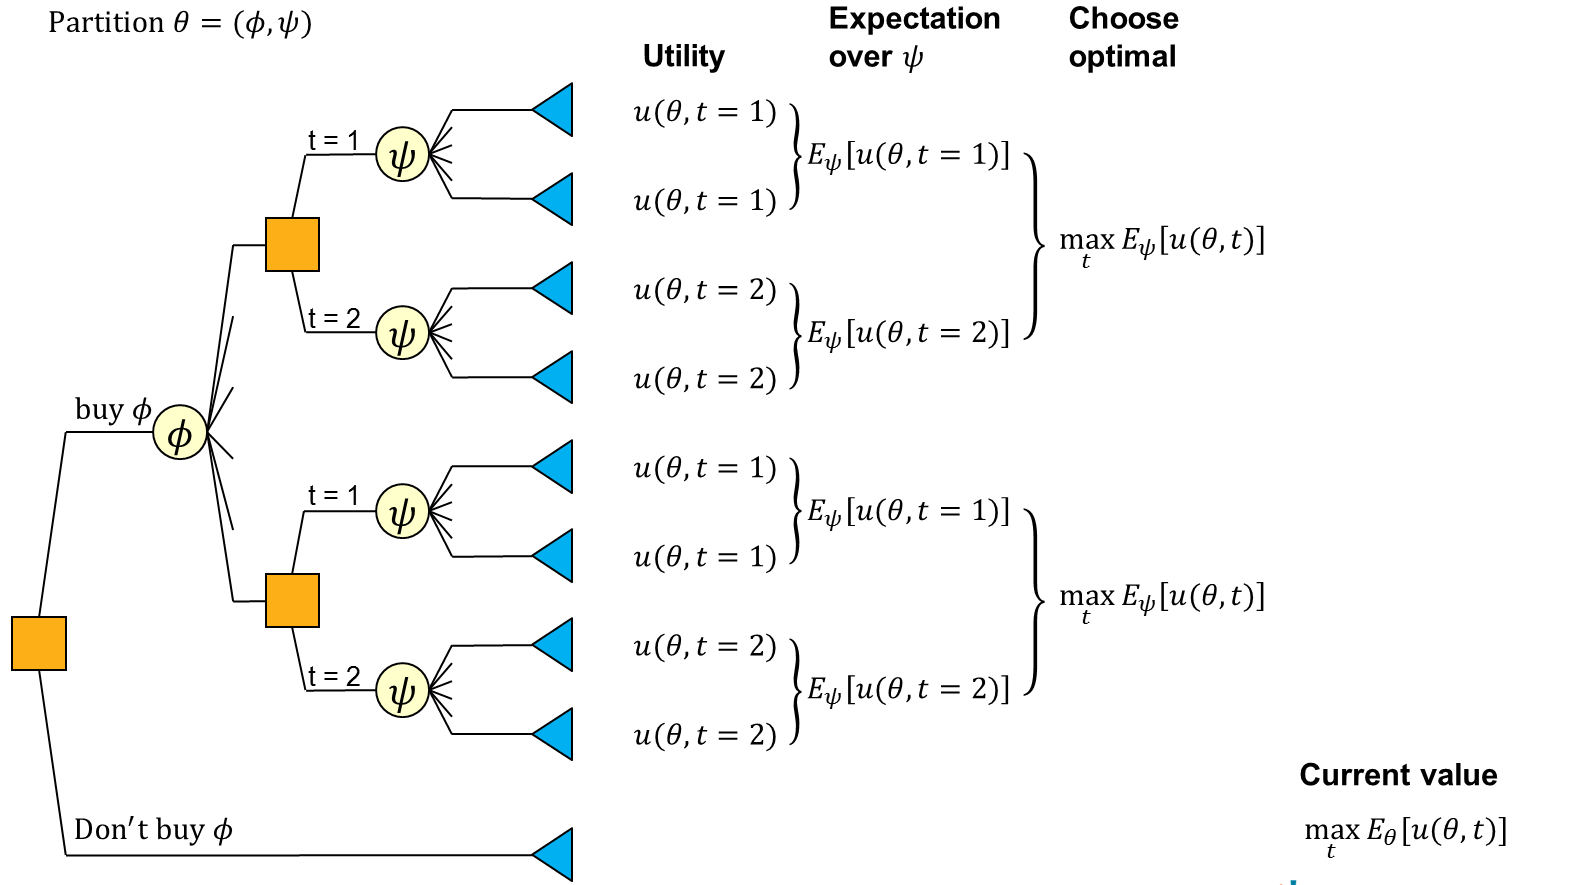
\includegraphics[height=6.5cm]{6.probabilistic-sensitivity-analysis/figs/EVPPI6.png}}}
%%%%%%%%%%%\only<7->{\put(0,0){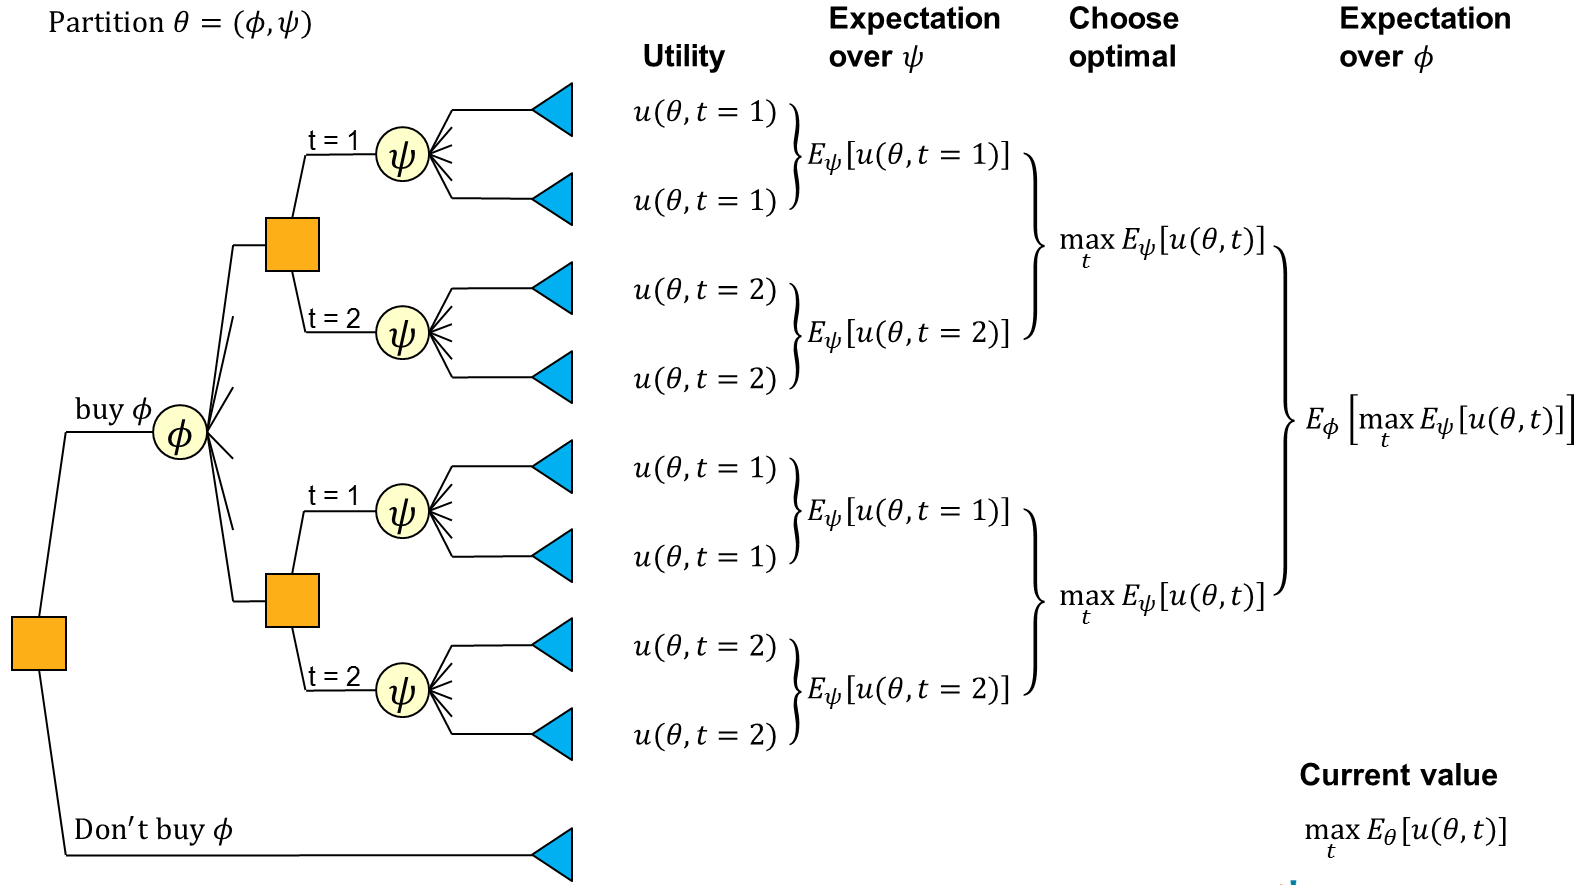
\includegraphics[height=6.5cm]{6.probabilistic-sensitivity-analysis/figs/EVPPI7.png}}}
%%%%%%%%%%%\end{overpic}
%%%%%%%%%%%\end{center}
%%%%%%%%%%%
%%%%%%%%%%%
%%%%%%%%%%%\end{frame}
%%%%%%%%%%%
%%%%%%%%%%%%### New page ############################################################
%%%%%%%%%%%
%%%%%%%%%%%\begin{frame}[fragile]
%%%%%%%%%%%
%%%%%%%%%%%\frametitle{How to estimate EVPPI by simulation}
%%%%%%%%%%%
%%%%%%%%%%%{\small
%%%%%%%%%%%$\theta$ is partitioned into $(\phi, \psi)$\\
%%%%%%%%%%%Decision to buy information on $\phi$\\
%%%%%%%%%%%1) Simulate a set of parameters $\mathbf{\phi} = \phi_1 ,\ldots, \phi_I$\\
%%%%%%%%%%%
%%%%%%%%%%%2) For each parameter $\phi_i$\\
%%%%%%%%%%%
%%%%%%%%%%%    \hspace{1em} a) Simulate a set of parameters $\mathbf{\psi} = \psi_1 ,\ldots, \psi_J$\\
%%%%%%%%%%%
%%%%%%%%%%%    \hspace{1em} b) For each treatment $t_k = t_1, \ldots , t_K$\\
%%%%%%%%%%%
%%%%%%%%%%%        \hspace{2em} i) Find utility of treatment $t_k$ for each $\psi_j$. $u(\phi_i, \psi_j, t_k)$\\
%%%%%%%%%%%        \hspace{2em} ii) Estimate $\mathbb{E}_{\psi}\left[u(\phi_i, \psi, t_k)  \right]$ by the mean over $j$ of $u(\phi_i, \psi_j, t_k)$\\
%%%%%%%%%%%
%%%%%%%%%%%    \hspace{1em} c) Choose treatment $t^*$ that is $max_t \mathbb{E}_{\psi}\left[u(\phi_i, \psi, t_k)  \right]$
%%%%%%%%%%%
%%%%%%%%%%%3) Value of decision is $\mathbb{E}_{\phi}\left[\max_t \mathbb{E}_{\psi}\left[u(\phi, \psi, t)  \right] \right]$ which is estimated by the mean over $i$ of $\mathbb{E}_{\psi}\left[u(\phi_i, \psi, t^*)  \right]$\\
%%%%%%%%%%%
%%%%%%%%%%%\vspace{1em}
%%%%%%%%%%%\[
%%%%%%%%%%%\mbox{EVPPI} = \mathbb{E}_{\phi}\left[\max_t \mathbb{E}_{\psi}\left[u(\phi, \psi; t)  \right] \right] - \max_t\mathbb{E}_{\theta}\left[u(\theta; t)  \right]
%%%%%%%%%%%\]
%%%%%%%%%%%
%%%%%%%%%%%}
%%%%%%%%%%%
%%%%%%%%%%%\end{frame}
%%%%%%%%%%%
%%%%%%%%%%%%### New page ############################################################
%%%%%%%%%%%
%%%%%%%%%%%\begin{frame}[fragile]
%%%%%%%%%%%
%%%%%%%%%%%\frametitle{How to estimate EVPPI by simulation}
%%%%%%%%%%%
%%%%%%%%%%%{\footnotesize
%%%%%%%%%%%\bi
%%%%%%%%%%%\item This algorithm is extremely computationally intensive
%%%%%%%%%%%\item For every simulated value of $\phi$, we have to simulate a set of $\psi$'s
%%%%%%%%%%%\item And then repeat this for every parameter, and every WTP threshold
%%%%%%%%%%%\item This means this algorithm is practically infeasible, so approximations have been developed\footnote{\fontsize{7}{8}\selectfont Strong et al. (2013,2014). Sadatsafavi et al. (2013), Heath \& Baio (2015)}
%%%%%%%%%%%\item These algorithms only need a single set of parameter values, and the corresponding utility values for each treatment
%%%%%%%%%%%\item This is exactly what we get when simulating the expected NB for each treatment in \bugs
%%%%%%%%%%%\ei
%%%%%%%%%%%
%%%%%%%%%%%\begin{center}
%%%%%%%%%%%\begin{tabular}{rrrrrrrr}
%%%%%%%%%%%  \hline
%%%%%%%%%%% Simulation & $\pi_1$ & $\rho$ & $\gamma$ & $c^{\rm{amb}}$ & $c^{\rm{hosp}}$ & $NB_1$ & $NB_2$ \\
%%%%%%%%%%%  \hline
%%%%%%%%%%%1 & 0.15 & 0.73 & 0.62 & 106 & 5 410 & 3 654 900 & 4 049 100 \\
%%%%%%%%%%%  2 & 0.23 & 0.78 & 0.57 & 146 & 4 705 & 3 259 200 & 3 134 300 \\
%%%%%%%%%%%  3 & 0.28 & 0.72 & 0.65 & 113 & 5 858 & 3 095 200 & 3 041 100 \\
%%%%%%%%%%%  4 & 0.27 & 0.74 & 0.62 & 99 & 6 448 & 2 588 300 & 2 755 000 \\
%%%%%%%%%%%  5 & 0.24 & 0.89 & 0.44 & 107 & 5 225 & 2 968 300 & 2 778 000 \\
%%%%%%%%%%%   \hline
%%%%%%%%%%%\end{tabular}
%%%%%%%%%%%\end{center}
%%%%%%%%%%%}
%%%%%%%%%%%
%%%%%%%%%%%\end{frame}
%%%%%%%%%%%
%%%%%%%%%%%%### New page ############################################################
%%%%%%%%%%%
%%%%%%%%%%%\begin{frame}[fragile]
%%%%%%%%%%%
%%%%%%%%%%%\frametitle{Estimating EVPPI by regression (recommended method)}
%%%%%%%%%%%
%%%%%%%%%%%\[
%%%%%%%%%%%\mbox{EVPPI} = \mathbb{E}_{\phi}\left[\max_t \mathbb{E}_{\psi}\left[NB(\phi, \psi; t)  \right] \right] - \max_t\mathbb{E}_{\theta}\left[NB(\theta; t)  \right]
%%%%%%%%%%%\]
%%%%%%%%%%%
%%%%%%%%%%%General principle {\footnotesize (Strong et al., Medical Decision Making 2014)}
%%%%%%%%%%%
%%%%%%%%%%%\begin{itemize}
%%%%%%%%%%%
%%%%%%%%%%%\item For each treatment $t$, fit a regression model of $NB_t$ on parameter(s) of interest $\phi$ using these simulations
%%%%%%%%%%%
%%%%%%%%%%%\item Take the \alert{mean over simulations} of \alert{maximum over $t$} of \emph{fitted values} $E(NB_t | \phi)$ from these regressions
%%%%%%%%%%%
%%%%%%%%%%%\item This is an estimate of $\mathbb{E}_{\phi}\left[\max_t \mathbb{E}_{\psi}\left[NB(\phi, \psi; t)  \right] \right]$
%%%%%%%%%%%
%%%%%%%%%%%\end{itemize}
%%%%%%%%%%%\pause
%%%%%%%%%%%Implemented in
%%%%%%%%%%%\begin{itemize}
%%%%%%%%%%%\item SAVI web application \url{http://savi.shef.ac.uk/SAVI} {\footnotesize (Strong et al.)}
%%%%%%%%%%%\item BCEA R package {\footnotesize (Heath \& Baio 2015)} 
%%%%%%%%%%%\end{itemize}
%%%%%%%%%%%
%%%%%%%%%%%via various non-parametric, non-linear regression methods: ongoing work to find the most reliable$\ldots$
%%%%%%%%%%%
%%%%%%%%%%%\end{frame}
%%%%%%%%%%%
%%%%%%%%%%%
%%%%%%%%%%%%### New page ############################################################
%%%%%%%%%%%
%%%%%%%%%%%\begin{frame}[fragile]
%%%%%%%%%%%
%%%%%%%%%%%\frametitle{EVPPI plot}
%%%%%%%%%%%
%%%%%%%%%%%\begin{center}
%%%%%%%%%%%\rotatebox{0}{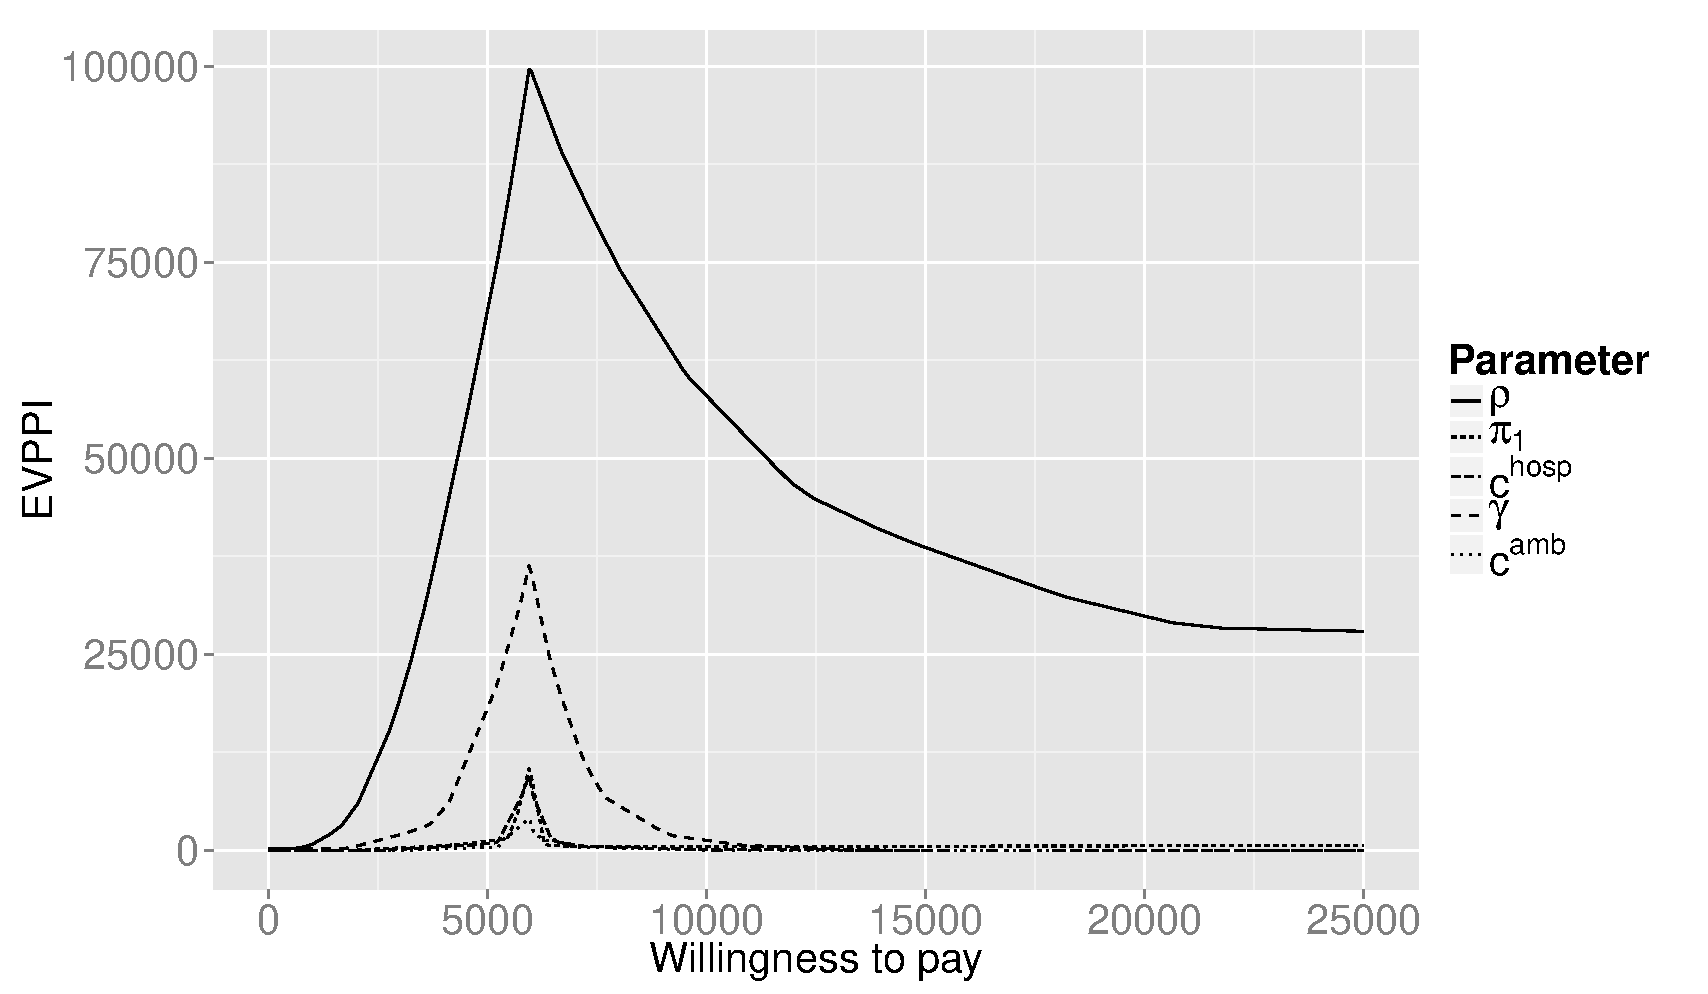
\includegraphics[height=4.5cm]{6.probabilistic-sensitivity-analysis/figs/chemo_EVPPI.pdf}}
%%%%%%%%%%%\end{center}
%%%%%%%%%%%
%%%%%%%%%%%{\footnotesize
%%%%%%%%%%%\bi
%%%%%%%%%%%\item The greatest value in reducing parameter uncertainty are from the parameters
%%%%%%%%%%%    \bi
%%%%%%%%%%%    \item $\rho$ Probability of side effect given new treatment compared to SoC
%%%%%%%%%%%    \item $\pi_1$ Probability of side effect given SoC
%%%%%%%%%%%    \ei
%%%%%%%%%%%\item There is relatively little value in reducing the uncertainty in the other parameters
%%%%%%%%%%%\ei
%%%%%%%%%%%}
%%%%%%%%%%%
%%%%%%%%%%%\end{frame}
%%%%%%%%%%%
%%%%%%%%%%%%### New page ############################################################
%%%%%%%%%%%
%%%%%%%%%%%\begin{frame}
%%%%%%%%%%%
%%%%%%%%%%%\frametitle{Conclusions}
%%%%%%%%%%%
%%%%%%%%%%%\bi
%%%%%%%%%%%\item Using \bugs for PSA
%%%%%%%%%%%    \bi
%%%%%%%%%%%    \item Set up a deterministic model
%%%%%%%%%%%    \item ``Push through'' the uncertainty in the parameters to uncertainty in the model outputs
%%%%%%%%%%%    \ei
%%%%%%%%%%%\item Define ICER, INB, CEAC
%%%%%%%%%%%\item How to find these in \bugs
%%%%%%%%%%%\item Define and calculate EVPI and EVPPI
%%%%%%%%%%%\ei
%%%%%%%%%%%
%%%%%%%%%%%\end{frame}
%%%%%%%%%%%
%%%%%%%%%%%\begin{frame}
%%%%%%%%%%%
%%%%%%%%%%%  \frametitle{Practical: Probabilistic sensitivity analysis in BUGS}
%%%%%%%%%%%
%%%%%%%%%%%  \textbf{There are three questions in this practical which can be done in any order}
%%%%%%%%%%%
%%%%%%%%%%%  \begin{itemize}
%%%%%%%%%%%
%%%%%%%%%%%  \item Question 1) is about running the chemotherapy model in BUGS. This is the easiest question. Do this if you want more practice in using BUGS.
%%%%%%%%%%%
%%%%%%%%%%%  \item Question 2) is about understanding value of information, and does not use BUGS.
%%%%%%%%%%%
%%%%%%%%%%%  \item Question 3) is about interfacing BUGS with R using the package \texttt{R2OpenBUGS}, and drawing figures and performing EVPPI calculations using the package \texttt{BCEA}.
%%%%%%%%%%%
%%%%%%%%%%%  \end{itemize}
%%%%%%%%%%%
%%%%%%%%%%%\end{frame}
%%%%%%%%%%%
%%%%%%%%%%%